\documentclass[12pt]{article}
\usepackage{graphicx} % Requiredwargawwwwww for inserting images
\usepackage[a4paper, top=2.5cm, bottom=2.5cm, left=3cm, right=3cm]%
{geometry}
\usepackage{fancyhdr}
\usepackage{amsmath}
\usepackage{ragged2e}
\usepackage{mathptmx}
\usepackage{setspace}
\usepackage{footnote}
\usepackage{footmisc}
\usepackage{float}
\usepackage{textcomp}
\usepackage[francais]{babel}
\renewcommand{\contentsname}{Sommaire}
\renewcommand{\thesection}{\Roman{section}} % Numérotation en chiffres romains
\pagestyle{fancy}

%Edition Entête
\fancyhead[C]{\leftmark}
\fancyhead[L]{COP-AMACO}
\fancyhead[R]{}

%Edition pied de page 
\fancyfoot[C]{Mémoire Licence professionnelle }
\fancyfoot[L]{Anthony Wilhelm}
\fancyfoot[R]{\thepage}


    
\title{Mémoire Licence pro 2023}
\author{Anthony Wilhelm }
\date{May 2023}

\begin{document}

\setstretch{1} % Définition de l'interligne à 1

\begin{titlepage}
\centering
\begin{flushright}
15 AOUT 2023\\[10pt]
\end{flushright}
\vfill
\begin{center}

\begin{figure}[h]
    \begin{minipage}[c]{.46\linewidth}
        \centering
        
\includegraphics{img/fstlogo.png}
       
    \end{minipage}
    \hfill%
    \begin{minipage}[c]{.46\linewidth}
        \centering
        
\includegraphics{img/uha4.0logo.png}
        
    \end{minipage}
\end{figure}
\end{center}
\begin{center}

\includegraphics{img/logoCop.png}
\end{center}
\vfill

\begin{center}
    
\begin{Large}
    \text {Création d'une application de maintenance prédictive }
\end{Large}\\[3pt]
    \text {Mémoire de Licence Professionelle developpement informatique 2023 } 
\end{center}
\vfill

   \begin{center}
   \justify
    \text{Promotion |  2022/2023}
\end{center}
\begin{center}
\justify
    \text {Diplome Universitaire | Licence Professionelle developpement informatique 2023}
\end{center}
\begin{center}
\justify
\text {Rédigé par |  Anthony WILHELM} 
\end{center}
\begin{center}
\justify
\text{Entreprise | COP-AMACO}    
\end{center} 
\begin{center}
\justify
\text{Tuteur professionnel | Franck LEMKE}    
\end{center} 
\begin{center}
\justify
\text{Tuteur Pédagogique | Mounir ELBAZ}    
\end{center} 
   



% \begin{flushleft}
% Relatório do Experimento 7  - Laboratório de Conversão Eletromecânica de Energia\\
% Professor André Guilherme Peixoto Alves\\
% Grupo 2\\
% Alunos:\\ 
%     \hspace{1cm}Gabriela Lemos\\
%     \hspace{1cm}Renan Pinho\\
%     \hspace{1cm}Rafael Almeida\\
%     \hspace{1cm}Gabriel Fávero\\

% \end{flushleft}

\vfill



\end{titlepage}

%biblio graphie 
    % def soft skils => le figaro https://emploi.lefigaro.fr/evolution-professionnelle/guide-de-l-evolution-professionnelle/61-soft-skills-definition-avantages-cv-et-formation/


\begin{titlepage}
    \centering
    \begin{Large}
        \text {Remerciement}  
    \end{Large}\\[3pt]
    
    \begin{justify} 
    \justify
	Je tiens à remercier toutes les personnes qui ont contribué à la réussite de mon alternance lors de ma 3e année et qui m'ont accueilli au sein de l'entreprise COP-AMACO.
    \justify
    Je souhaite adresser des remerciements spéciaux à M. Pascal BONETTO qui a eu confiance en moi en me permettant de rejoindre son équipe pour cette alternance.
    \justify
    Merci également à M. Franck LEMKE, mon responsable durant l'alternance, pour la qualité de son encadrement, sa disponibilité et la confiance qu'il m'a accordée.
    \justify
    Je tiens a également  toutes les personnes du service digital avec qui j'ai collaboré et acquis de nouvelles compétences tout au long de mon alternance, ce qui m'a permis de progresser dans le développement.
    \justify
    Je remercie aussi l'équipe enseignante de l'UHA 4.0 pour leur professionalisme dont ils ont fais preuve tout au long de mon parcours à l'UHA 4.0.

    \justify
    Enfin, je remercie toutes les personnes qui ont contribué en m'aidant dans la relecture de ce document. 
    
    \end{justify}
    
\newpage
\end{titlepage}
\thispagestyle{empty}
\tableofcontents


%Page d'intro

\newpage
\setcounter{page}{1} % Réinitialiser le compteur de pages à 1
\centering
\vspace{2cm}
\section*{Introduction}
\vspace{2cm}
\addcontentsline{toc}{section}{Introduction}
\markboth{INTRODUCTION}{INTRODUCTION}
\thispagestyle{empty} % Applique le style d'en-tête à la page d'introduction
\centering % Centre le titre "Introduction" dans l'en-tête

\justify
\text
Le mémoire que vous allez lire est le résultat d'un projet d'étude d'un an réalisé pendant mon alternance. Il marque également la fin de trois années consécutives d'études dans le domaine du developpement informatique.
\justify
\text
Pendant mon année chez COP-AMACO, j'ai eu l'opportunité de contribuer à plusieurs projets, notamment un premier projet visant à organiser le service après-vente de l'entreprise et un second visant à prévenir les pannes  des caisses de supermarché, avec ce projet nous voudrions répondre à plusieurs problématiques qui se posent pour les distributeurs.Dans un contexte de baisse générale du pouvoir d'achat, la majeur partie des distributeurs cherchent à réduire leur masse salariale pour rester compétitif.
\justify
\text Le remplacement d'une partie des lignes de caisses"standards" par des caisses libre service permet en partie d'atteindre cet objectif. Toutefois garder un nombre minimal de ligne de caisse classique demeure indispensable (PMR "Personne à mobilité réduite ",grande capacité d'achat), dès lors maintenir ces caisses en état de fonctionnement représente un enjeu important (les caisses étant en nombre limité, toute caisse hors-service représente un désagrément pour l'utilisateur notamment des temps d'attentes plus long). Pouvoir détecter les pannes(mécanique et électrique) de manière anticipée peut aider à maximiser le nombre de caisses utilisable. Dans ce document, je me concentrerai uniquement sur ce dernier projet .
\justify
\text
Je commencerai d'abord par présenter mon parcours personnel, puis je vous parlerai de l'entreprise. Ensuite, je vous présenterai le cahier des charges de projet ce baptisé "KMO-PREDICT" . Enfin je vous montrerai les travaux que j'ai réalisés sur ce projet.


\newpage

\section{Contexte}
Je vais décrire dans cette partie le contexte qui m'a permis de développer pour COP-AMACO. Je parlerai des étapes de mon parcours scolaire et professionnel, ainsi que des différents projets auxquels j'ai contribués.

Tout d'abord, je vais présenter la formation UHA 4.0 et son approche pédagogique. Ensuite, je présenterai mon expérience personnelle dans cette formation, et enfin, je parlerai de l'entreprise qui m'a accueilli pendant mon alternance .

\subsection{La formation}

\justify
\text
L'UHA 4.0 a une approche pédagogique basée sur l'apprentissage autonome de l'apprenant, en appliquant les connaissances acquises lors de projets encadrés par des enseignants issus du monde professionnel et apportés par des entreprises de toute la France. Les étudiants se forment par eux-mêmes  et suivent un plan de formation. Une année type à L'UHA 4.0 sans contrat de professionnalisation se décompose de la manière suivante : pendant les deux premiers mois de formation, nous nous formons grâce à un "Fil rouge".
\justify
\text
Le "Fil rouge" est un projet d'entraînement qui permet de mettre en pratique les connaissances acquises pendant la réussite de certifications du site OpenClassRoom. Il permet aussi aux enseignants d'évaluer le niveau de l'apprenant et de vérifier qu'il est en phase avec les connaissances attendues pour son année de formation.
\justify
\text
Ensuite, il y a deux projets de 6 semaines par groupe de 6-7 étudiants sur un projet apporté par une entreprise. Pour finir, des stages en entreprise d'une période de 6 mois sont effectués chaque année de formation. Ces projets ont pour but d'apprendre les méthodologies de la gestion de projets. Les étudiants des années supérieures approfondissent leurs connaissances dans la gestion de projet et mettent en pratique leurs compétences auprès des étudiants des années inférieures qui composent l'équipe et auprès de l'entreprise qui porte le projet (qui a le rôle de client). Il permet aux étudiants novices d'apprendre et d'observer le déroulement d'un projet informatique au sein de l'UHA 4.0.
\justify
\text
Cette partie de la formation est selon moi l'une des plus intéressantes, car elle permet de mettre en application directe les différentes notions apprises pendant les deux premiers mois de formation. Elle permet aussi aux étudiants des années supérieures de transmettre leur savoir aux étudiants des années inférieures dans des cas concrets. Les étudiants participants à cette phase de projets apprendront aussi ou perfectionneront leur travail en équipe ainsi que leurs compétences de communication, qui sont des SoftSkills cruciaux pour le bon déroulement de leurs futurs projets en entreprise en dehors de la gestion de projets.
\justify
\text
Ces deux phases de projets permettent à l'étudiant de mettre un premier pied dans la relation avec les entreprises (souvent de la région), ce qui peut aussi aider pour la recherche de stage. Il arrive souvent que les entreprises sélectionnent des étudiants ayant travaillé sur leur projet à l'école et leur permettent de le continuer en stage pendant une période de 6 mois, ce qui les plongera dans un cadre professionnel et leur fera acquérir de nouvelles compétences propres au milieu du travail.

\newpage
\justify
\text
Chaque année, nous nous formons sur un type de technologie ou de concept particulier. Pendant la première année, l'objectif est de former l'étudiant sur les technologies du web et les fondamentaux du développement. Nous apprenons des langages comme HTML/CSS, PHP, SQL et JavaScript. Nous nous familiarisons également avec certains outils tels que GIT pour la gestion des versions du code et Confluence pour la rédaction de documentation. Les élèves les plus rapides peuvent aussi apprendre des frameworks tels que Angular ou Symphony.
\justify
\text
 La deuxième année vise à élargir le champ de compétences de l'étudiant. Nous nous formons au concept de la programmation orientée objet en utilisant un langage objet de notre choix (C\#, JAVA, etc.). Les étudiants de 4.0.2 se forment également à la conception d'applications et à l'utilisation de frameworks. De plus, nous sommes introduits à la gestion de projet, c'est-à-dire comment découper un projet en tâches et reconnaître les fonctionnalités les plus importantes pour (le client Most Valuable Product M.V.P).
\justify
\text
Enfin, la dernière année de formation a pour objectif d'approfondir les compétences acquises les années précédentes et de permettre à l'étudiant de devenir acteur du cycle de développement du logiciel. La troisième année aborde les méthodologies pour mener un projet, ainsi que celles qui permettent de rendre un projet maintenable sur le long terme, en abordant les tests unitaires (et les tests automatisés pour les plus rapides). Le "Fil rouge" de la troisième année a la particularité de ne pas imposer de technologie aux étudiants, ce qui leur permet d'explorer des technologies non abordées les années précédentes, comme les bases de données non relationnelles ou le développement mobile.
\justify
\text
Le point commun à chaque année est une période de 6 mois de stage, au cours de laquelle les étudiants sont évalués grâce à un rapport de stage et une soutenance orale afin de valider le D.U de chaque année.

\subsection{Mon parcours Scolaire}
\justify
\text
Après avoir obtenu mon Baccalauréat scientifique en 2018, j'ai d'abord intégré la faculté des sciences techniques de Mulhouse en Licence Math et informatique en L12A, où je devais faire ma première année de licence en 2 ans.
\justify
\text
J'ai réussi à passer la première année, mais j'ai été contraint d'abandonner au cours de la 2ème année en raison de résultats insatisfaisants aux partiels pendant la période COVID. J'ai alors envisagé une réorientation, mais je voulais toujours rester dans le milieu de l'informatique, car la partie informatique de la licence m'avait vraiment plu, notamment le cours de développement web.
\justify
\text
En cherchant de l'aide pour me réorienter sur le campus, j'ai découvert l'UHA 4.0 grâce à une conseillère. Je lui ai parlé de mon envie d'études plus concrètes, et elle m'a conseillé de rejoindre l'école ou de faire un BTS SIO. À ce moment-là, j'ai rencontré un stagiaire de l'UHA 4.0, et nos discussions m'ont convaincu de rejoindre l'école. J'ai donc intégré l'école en septembre 2020 en 1ère année.
\justify
\text
J'ai ensuite suivi trois années à l'école, mêlant apprentissage en autonomie, projets concrets et immersion en entreprise lors des stages effectués ainsi que une alternance. Je vais maintenant détailler les projets que j'ai effectués au sein de l'école UHA 4.0 par ordre chronologique, en expliquant rapidement leur contexte et mes contributions sur chacun d'eux.

\newpage

\subsubsection{1\textsuperscript{ère} année}

\begin{itemize}
\item \textbf{ELAN}
    \newline Le projet ELAN était porté par l'UHA et avait pour objectif d'aider les étudiants lycéens à trouver une formation parmi celles proposées à l'université. Pour cela, une application web a été développée avec un quizz permettant de proposer une liste personnalisée de formations et de renvoyer les utilisateurs vers des fiches explicatives sur les différentes options disponibles. En somme, ELAN visait à devenir un "GPS des formations".\footnote{Une application web qui aide les étudiants à trouver leur formation idéale.}

    \newline Mes contributions sur ce projet ont consisté à rendre l'application responsive, c'est-à-dire adaptée à différents appareils, et à créer l'espace administrateur dans le front-end en utilisant le CRUD de l'API développée par mes camarades des années supérieures.\footnote{CRUD signifie Create, Read, Update, Delete. C'est un ensemble d'opérations basiques pour les applications qui gèrent les données.}

     \newline Ce fut ma première expérience de projet, au cours de laquelle j'ai pu découvrir les frameworks NestJS et Angular, ainsi que la méthode de gestion de projet AGILE avec le framework SCRUM, qui attribue différents rôles et tâches spécifiques aux différentes parties prenantes du projet.\footnote{AGILE est une approche souple et itérative de la gestion de projet, et SCRUM est l'un de ses frameworks les plus populaires.}
    
    \item \textbf{Edeina}
   
        \newline Le projet Edeina a pour but de créer une application permettant de partager des informations sur les patients et leur dossier médical au sein de l'association Edeina. De plus, l'application permet aux patients de trouver facilement des praticiens membres de l'association. Les technologies utilisées pour ce projet sont NestJS et Angular.

        \newline Dans ce projet, j'ai contribué à la création du profil des patients, à la mise à jour des données du patient, ainsi qu'à la vue patient accessible par les praticiens. J'ai également ajouté des entrées dans la base de données et créé une méthode Update dans le back-end (la partie du logiciel qui produit les résultats et qui est opposée au front-end, la partie visible de l'application).

        \newline Ce projet m'a permis de découvrir une partie que je n'avais pas encore expérimentée, le back-end, c'est-à-dire la partie du logiciel qui gère les données et les traitements en arrière-plan.
    
    \item \textbf{Stage association Brunstatt-didenheim-artisant-commençant} 
   
        \newline Lors de mon premier stage de 4 mois, j'ai été accueilli par une association qui souhaitait que je développe leur site vitrine pour promouvoir les commerçants et artisans des deux villages. Le site devait présenter chaque membre de l'association, comporter un espace administrateur pour gérer l'affichage des membres et pouvoir ajouter des annonces sur la page principale du site. J'ai également dû déployer l'application sur le serveur de l'hébergeur choisi par l'association. J'ai utilisé les technologies NESTJS et Angular, ainsi qu'une base de données MySQL pour réaliser le site web.

       \newline En tant que seul développeur sur le projet, j'ai beaucoup appris à travailler en autonomie et j'ai acquis énormément de compétences à la fois dans le back-end et le front-end.

        \newline À la fin du stage, j'avais produit un site web fonctionnel et esthétique que j'ai déployé sur un serveur et mis à disposition de l'association. Les enseignements que j'ai pu tirer de ce stage sont l'importance de bien cerner les besoins et les demandes des utilisateurs, ainsi que de faire des recherches sur les différentes technologies avant de se lancer dans le code, afin de ne pas surdimensionner le projet.
\end{itemize}


\subsubsection{2\textsuperscript{ème} année}
\begin{itemize}
    \item \textbf{M2A}
    \newline La demande du client était de créer une application web sous forme de jeux sérieux, destinée à des personnes ne sachant pas utiliser un ordinateur ni connaître l'utilisation du clavier et de la souris. Pour ce projet, nous avons utilisé uniquement la technologie Blazor un framework front-end basé sur le C\#, car l'application ne nécessitait pas d'API\footnote{Interface de programmation d'application utilisée généralement pour réaliser la partie backend des projets web. Elle regroupe les différentes méthodes et fonctions qui manipulent la base de données.}. Cependant, nous devions conserver une persistance modérée des données (environ une journée) sans aucune authentification, en stockant les données de l'utilisateur dans son navigateur.
    \newline  Sur ce projet, j'ai créé un jeu avec plusieurs niveaux pour apprendre aux utilisateurs à utiliser la souris, en utilisant le clic droit, le clic gauche et le déplacement. Pour cela, j'ai dû différencier un clic droit d'un clic gauche et mettre en place un système de placement aléatoire des boutons dans un espace en deux dimensions. J'ai également mis en place la sauvegarde de la progression de l'utilisateur avec des cookies, en créant une structure de données pour stocker toute la progression dans un cookie.

    \newline  Grâce à ce projet, j'ai pu expérimenter la technologie Blazor, ce qui m'a permis de découvrir le langage C\# et l'environnement de développement de Dotnet. J'ai également découvert le développement de jeux.

    \item \textbf{Epromoove}
     \newline L'entreprise qui nous a confié ce projet se spécialise dans la conception de systèmes mécatroniques et robotiques pour les professionnels du BTP. L'objectif du projet était de récupérer les données produites par les robots (tension de la batterie, vitesse du moteur, etc.) et de les stocker dans une base de données. Ensuite, ces données devaient être traitées et renvoyées vers une application web. Les technologies utilisées pour ce projet étaient Angular pour la partie client, NestJS pour la partie serveur, ainsi que MongoDB pour la récupération des données brutes, couplé avec une base de données MySQL pour les données triées.

     \newline Pendant ce projet, j'ai contribué à la mise en place de l'envoi de données en C++ vers le serveur web. J'ai également participé à la création de l'API et à la mise en place des bases de données.

      \newline Ce projet m'a permis de découvrir les bases de données NoSQL ainsi que le langage C++. J'ai également appris à gérer une grande quantité de données.
    \item \textbf{Stage COP-AMACO}
        \newlineJ'ai été accueillie dans l'entreprise COP-AMACO pour une durée de 6 mois. COP-AMACO conçoit des meubles pour aménager les espaces de vente et des lignes de caisses pour la grande distribution. Mon stage avait pour objectif de développer un outil de ticketing et de créer des rapports d'intervention électroniques pour la gestion du service après-vente de l'entreprise. J'ai participé au développement de l'API avec la technologie NESTjs, au client web avec Angular, ainsi qu'à l'application mobile utilisée par les techniciens pour remplir les rapports sur le terrain, développée avec la technologie IONIC. Cette application doit permettre au service SAV de suivre l'état des demandes d'intervention, faciliter la facturation des interventions et supprimer les versions papier des rapports. Elle servira également à assurer la traçabilité des SAV dans les différents magasins et à fournir des statistiques pour justifier les coûts des SAV aux clients de l'entreprise.

        \newline  Pendant ce stage, j'ai collaboré avec un autre stagiaire développeur pour concevoir l'application. J'ai pu mettre en pratique les connaissances acquises pendant les phases de projet sur la gestion du travail en équipe. Nous avons régulièrement organisé des réunions avec les techniciens du service SAV pour bien comprendre leurs besoins, ce qui m'a beaucoup appris sur la manière de comprendre les exigences techniques de personnes qui ne maîtrisent pas nécessairement les outils informatiques.

        \newline À la fin du stage, une application mobile, un site web, une API et une base de données (MYSQL) ont été déployés grâce à Docker. Nous avons pu effectuer des tests sur le terrain avec les monteurs, qui ont été très concluants. Aujourd'hui, l'application est en cours d'adoption par les salariés de l'entreprise, et son utilisation, qui pour l'instant se limite au Grand-Est, devrait s'étendre à tous les monteurs de l'entreprise.

        \newline L'entreprise s'est montrée satisfaite de mon travail et m'a permis de continuer en contrat de professionnalisation pour ma 3\textsuperscript{ème} année.
    
    
\end{itemize}
\subsubsection{3\textsuperscript{ème} année}
\begin{itemize}
    \item  \textbf{Alter-Alsace}
        \newline L'entreprise Alter Alsace est une association qui vise à mesurer la consommation d'eau et d'énergie des bâtiments publics des communes d'Alsace. Le projet consistait à reprendre une application existante utilisée par des experts ou des responsables de communes pour contrôler les consommations des bâtiments. L'association souhaitait une refonte de la base de données pour éviter les redondances qui ralentissaient l'application. Ils voulaient également que les utilisateurs puissent entrer manuellement les données de consommation des bâtiments.

         \newline Le projet utilisait les technologies suivantes : NodeJS et MySQL pour le backend, et VueJS pour le frontend. Le code du projet était chaotique, car plusieurs stagiaires débutants avaient développé dessus avec peu de documentation. Pour rendre le code plus structuré et durable, nous avons conservé le frontend en VueJS et remplacé NodeJS par NestJS, un framework de NodeJS.

         \newline Pendant ce projet, j'ai participé à l'initialisation de la nouvelle API et à la création de la nouvelle base de données après la refonte. J'ai mis en place Docker pour faciliter la configuration de l'environnement de développement et simplifier le déploiement ultérieur. J'ai également intégré certaines fonctions mathématiques sous les conseils de l'expert analyste de l'énergie, puis j'ai relié les formules du backend aux courbes affichées dans le frontend.

        \newline Ce projet m'a permis de découvrir le processus de passage d'une version 1 du projet à une version 2, et l'importance de bien documenter et indenter le code. J'ai également appris à travailler en collaboration avec un expert dans son domaine pour intégrer l'intelligence qu'il souhaitait apporter à l'application.
    \item \textbf{Chalet}
         \newline Le projet "Chalet" avait pour objectif de créer le back-office d'un site web de location de chalets. L'idée était de permettre à l'administrateur du site de ne plus devoir modifier directement les informations en base de données, mais d'utiliser les routes de l'API du site web créée par le client. Notre tâche consistait à développer la partie front-end du back-office en utilisant C\# et Blazor. Le client nous a fourni une API de développement pour pouvoir tester le projet sur les serveurs de l'UHA 4.0.

        \newline  Sur ce projet, j'ai principalement travaillé sur la gestion du projet. Comme le projet était plus petit que prévu, j'ai mis l'accent sur la documentation pour faciliter la reprise du projet par le client. Beaucoup des étudiants avec nous n'avaient pas encore utilisé le C\# ni Blazor, donc j'ai pris en charge leur accompagnement et leur formation pour qu'ils comprennent le fonctionnement de ces technologies.

        \newline Ce projet m'a permis de perfectionner mes compétences en gestion de projets ainsi que dans l'utilisation des technologies C\# et Blazor.

    \item \textbf{Alternance chez COP-AMACO}
         \newline Pour clôturer ma troisième année de licence, j'ai effectué une alternance dans l'entreprise COP-AMACO, située à Nordhouse dans le Bas-Rhin, en France. Pendant cette année en alternance, j'ai été activement impliqué dans les différents projets de l'équipe digitale. Dans la suite de ce mémoire, je détaillerai en particulier mes développements, notamment sur l'un des projets menés par l'équipe digitale de COP-AMACO, dont je faisais partie.
\end{itemize} 

\subsection{COP-AMACO}
\justify
\text
COP-AMACO est une entreprise fondée en 1989 et actuellement dirigée par  Pascal Bonetto et basée à Nordhouse, en France. Cette société est spécialisée dans la conception et la fabrication de meubles et de caisses pour les espaces de vente, en particulier pour les grandes surfaces et les supermarchés. Son objectif est de créer des solutions fonctionnelles et esthétiquement attrayantes pour aider les détaillants à optimiser l'aménagement de leurs magasins et à améliorer l'expérience d'achat des clients.


\begin{figure}[H]
    \centering
    \includegraphics[width=\textwidth]{img/exempleDeRéalisation.drawio.png}
    \caption{Exemple de réalisation de l'entreprise}
    \label{fig:enter-label}
\end{figure}
\justify
\text
L'entreprise jouit d'une solide réputation dans l'industrie et a développé un portefeuille de projets réussis avec différents clients du secteur de la vente au détail.  Les produits de COP-AMACO vont des présentoirs et étagères aux comptoirs de caisse et aux guichets de service client.
\justify
\text
En plus de ses produits physiques, COP-AMACO s'est récement tournée vers le numérique à l'automne 2021 en mettant en place une équipe digitale. Cette équipe est chargée de développer des solutions innovantes qui combinent des éléments physiques et numériques pour améliorer  davantage l'expérience d'achat en magasin ainsi que sa gestion.
\justify
\text
Pendant mon alternance au sein de l'équipe digitale de COP-AMACO, j'ai eu l'occasion de travailler sur différents projets impliquant la création d'applications web et d'applications mobiles, ainsi que l'intégration de solutions numériques dans leurs produits existants. 

%\footnote{L'Internet des objets (IoT) est %l'interconnexion entre Internet et des objets, lieux %et environnements physiques.} pour rendre les %produits plus connectés et interactifs.
\justify
\text Le Projet KMO-PREDICT fait partie du développement d'un portail SaaS (Software-as-a-Service), qui est une plateforme en ligne proposant des services logiciels accessibles via Internet. Ce type de service offre diverses fonctionnalités sans nécessiter d'installation ou de gestion locale du logiciel. Les avantages incluent une facilité d'utilisation, une grande flexibilité, une évolutivité et une tarification adaptable. Cependant, il est essentiel de prendre en compte la sécurité et la confidentialité des données lors du choix d'un fournisseur de services SaaS.

\begin{figure}[H]
    \centering
     \includegraphics[width=\textwidth]{img/sass_shéma.png}
    \caption{Schéma du futur portail SaaS de COP-AMACO}
    \label{fig:enter-label}
\end{figure}
    
   


\begin{itemize}
    \item [$\bullet$] Le projet KMO-PREDICT vise à permettre aux dirigeants de magasin d'anticiper les pannes et de vérifier l'état des lignes de caisse afin de planifier les maintenances au moment opportun. Il aidera également à améliorer la rapidité des interventions  en remontant les problèmes à COP-AMACO et en indiquant la nature de la panne.
    \item[$\bullet$] Le projet KMO-VIDEO vise à permettre aux dirigeants de magasin de gérée les différentes vidéo publicitaire qu'ils diffusent dans leur espace de vente afin de facilement pouvoir modifier cette dernière. 
    \item[$\bullet$] Le projet ATMOS a pour objectif de permettre dirigean de magasin  de gérer l'ambiance sonore de leurs magasins afin de diffuser des messages publicitaires audio ou des informations concernant le magasin.  
\end{itemize}

\newline
\justify
\text  J'ai  pour responsabilité, avec deux autres collègues, de développer et maintenir les différentes applications web.


\section{Cahier des charges }
\text Dans cette partie, je vais décrire les enjeux du projet KMO-PREDICT pour l'entreprise, les besoins qu'il va satisfaire pour les clients de l'entreprise, ainsi que les moyens mis en place pour mener le projet à bien.Je ne pourrais pas vous présenté un état existant du projet car il s'agit d'un tout nouveau projet initié lors de mon alternance.  

\subsection{Présentation du Projet KMO-PREDICT}
\justify
\text Le Projet KMO-PREDICT a débuté en février 2023. COP-AMACO fabrique des lignes de caisses pour les magasins de la grande distribution. Il arrive que ces caisses tombent en panne à force d'utilisation, et cela peut ne pas arriver au moment le plus opportun.L'application KMO-PREDICT est un projet de maintenance prédictive sur les caisses, qui permettra aux clients de planifier des services après-vente (SAV) avant que les caisses ne tombent réellement en panne.L'intérêt de ce projet est également important pour l'entreprise, car la caisse sera capable de signaler des erreurs et de cibler leurs sources. Le projet a plusieurs objectifs à court terme pour l'équipe :
\begin{itemize}
 \item [$\bullet$] Mettre en place le système IOT qui permettra d'alimenter l'API en données provenant des caisses.
\item [$\bullet$] Développer l'algorithme décisionnel qui déterminera si une intervention de maintenance est nécessaire en fonction des données collectées par le système IOT.
\item [$\bullet$] Permettre aux gestionnaire du magasin d'avoir un aperçu de leur parc de caisses par le biais d'une interface web.
\item [$\bullet$]  Permettre à un administrateur de COP de gérer les utilisateurs.
\item [$\bullet$] Avoir une version beta utilisable en 6 mois pour la tester dans un premier magasin pilote.
\end{itemize}

\subsection{Contraintes techniques de KMO-PREDICT}
\justify
\text Je vais définir ici uniquement les contraintes techniques pour la partie web du projet :

\justify
\text Un serveur doit être créé en utilisant le server nodeJS pour collecter les données de la "gateway" dans ce document quand je parlerais de "gateway", il s'agira de la carte electronique qui fais le lien entre la partie web et IoT du projet car "gateway" est le nom que nous avons attribué à cette carte . Ce serveur doit être sécurisé, extensible et capable de gérer plusieurs connexions en même temps. Il doit également réceptionner les données émises par des boitiers de contrôle des caisses et transmises par la "gateway", ainsi que répondre aux requêtes de l'interface utilisateur.

\justify
\text Une interface utilisateur intuitive sera développée pour visualiser l'état de maintenance des caisses et les résultats de l'analyse. Le choix de la technologie reste assez libre pour cette partie du projet.
De plus, cette plateforme doit intégrer un moyen pour la société COP-AMACO de gérer les magasins utilisant la solution (ajouter, supprimer, mettre à jour), ainsi que permettre à l'administrateur d'appareiler les "gateways" et les magasins.

\justify
\text Un algorithme en Python doit être implémenté pour analyser les données collectées et déterminer si une caisse nécessite la programmation d'une intervention de maintenance ou non. L'algorithme ce basera sur les données de capteurs intégrés à la  caisse ainsi que sur sa durée total de fonctionnement ( certains composant d'usure doivent être changés tous les 10 000h  de fonctionnement)afin déceler les anomalies que pourrais rencontré la caisse. Lorsqu'une telle intervention est préconisée, les données remontées par le systeme seront analysées pour déterminer les opérations que devront réaliser les techniciens sur site

\justify
\text Le système doit enregistrer des logs pour chaque caisse surveillée (soit environ plusieur centaine  de données à enregistrer dans la base de donnée toutes les minute pour chaque caisses monitorées), afin de permettre une analyse ultérieure des pannes par les techniciens du service après-vente. Les logs devront contenir des informations détaillées sur les données collectées, les résultats de l'analyse et toute autre information pertinente pour comprendre les raisons des pannes.
\justify
\text Le projet doit être intégré au portail SaaS des applications de l'entreprise gérée par Keycloak. Keycloak est un système open source de gestion d'identité et d'authentification développé par Red Hat. Il facilite la centralisation des identifications utilisateurs, offre du Single Sign-On (SSO) et supporte des protocoles comme OpenID Connect et SAML 2.0. Il permet aux applications de déléguer la gestion de l'authentification de manière sécurisée. Il permettra de gérer facilement et de façon sécurisée les droits d'accès dans l'application.

\subsection{Environnement de développement} 

\justify
\text Afin de gérer le projet, permettre à l'équipe de développement de s'organiser pour construire le projet, de suivre efficacement l'avancement et de faciliter le développement, nous avons utilisé plusieurs outils de gestion de projet. Je vais vous présenter les outils que nous avons utilisés pour développer KMO-PREDICT : 
\begin{itemize}

    \item [$\bullet$] Git est un outil de versionnage qui permet de créer différentes versions du projet. Pour partager le code au sein de toute l'équipe, nous avons utilisé GitHub. GitHub est un site web de gestion de code source dans le cloud qui permet aux développeurs de partager leur code et de rassembler plus facilement le travail effectué par chacun de leur côté. GitHub nous permet également de lancer des tests automatiques pour nous assurer qu'aucune régression n'est observée au fur et à mesure de l'ajout des fonctionnalités.
    
    \item [$\bullet$]Les IDE\footnote{Environnement de développement intégré} utilisés pour le développement de l'application KMO-PREDICT sont WebStorm, qui est particulièrement adapté aux technologies web en langage JavaScript et TypeScript comme NESTjs et Angular, ainsi que Visual Studio Code, un IDE gratuit permettant le développement sous tout type de langage, à condition d'être bien configuré. Sur ce projet, le choix de l'IDE dépend surtout de l'appréciation du développeur.
    
    \item [$\bullet$] Jira est un outil qui permet de découper le projet en différentes tâches qui pourront être planifiées et priorisées. Cet outil est très pratique pour le chef de projet, car il permet aussi de suivre l'évolution et l'avancement des tâches. Jira possède plusieurs états pour les différents tickets : "à faire", "en cours" et "terminé". Le chef de projet a ainsi une vue globale de l'avancement du développement de l'application.
    \item [$\bullet$] AWS (Amazon Web Services) est un ensemble d'outils que nous utilisons principalement pour héberger nos applications web et les rendre accessibles à nos clients. AWS a également une autre utilité, qui est de stocker une grande quantité de données à moindre coût et de les analyser grâce au service Lambda (exécution de code serverless) afin de renvoyer l'état de maintenance des caisses ou encore d'utiliser EC2, un service de serveur privé virtuel, pour mettre notre application à disposition.
\end{itemize}
\justify
\text Ces outils permettent donc la prévision, le développement et le déploiement de ce projet.

Nous avons choise de développer une  application web car elle présente plusieurs avantages :
\justify
\text L'utilisation d'une application web offre une plus grande portabilité que les applications natives. Les applications web sont, en effet, conçues pour fonctionner sur des navigateurs web couramment utilisés tels que Google Chrome, Mozilla Firefox, Safari, etc. Cela permet aux utilisateurs d'accéder à l'application depuis n'importe quel système d'exploitation (Windows, macOS, Linux) sans nécessiter de développement spécifique pour chaque plateforme. En conséquence, le développement et la maintenance de l'application web peuvent être simplifiés, car les développeurs n'ont pas à se soucier des différences de compatibilité entre les systèmes d'exploitation et les navigateurs.
\justify
\text Une application web offre une facilité de déploiement et de mise à jour. Étant donné que l'application est hébergée sur un serveur central, il est plus facile de déployer les mises à jour et les correctifs nécessaires. Les utilisateurs n'ont pas besoin de télécharger et d'installer manuellement les mises à jour, car celles-ci sont automatiquement disponibles lorsqu'ils accèdent à l'application. Cela garantit que tous les utilisateurs utilisent la dernière version de l'application sans avoir à gérer des installations ou des mises à jour complexes.
\justify
\text Cependant, il est important de noter que les applications web peuvent rapidement être limitées en therme de fonctionnalités par rapport aux applications natives . Les applications web doivent s'exécuter dans un navigateur, ce qui peut entraîner une surcharge et des performances légèrement inférieures.

\subsection{Choix de l'architecture et des technologies de l'application}

\justify
\text Le choix des différentes technologies pour cette application à pour but de gardée une certaine uniformisation dans les technologies utilisées dans le développement des l'applications de COP-AMACO.
\justify
\text Pour des raisons de performances et de flexibilité, l'application se décompose en trois partie parties :

\justify
\text Une partie serveur est développée en TypeScript avec le framework NESTjs pour Node.js. Cette technologie a été choisie car Node.js est un serveur bien connu par la plupart des développeurs web. NestJS et nodeJS jouissent d'une grande communauté ce qui permet d'avoir une grande variétée de documentation à disposition.NestJs apporte une architecture robuste ("MVC" Model View Controller) au projet de l'api ce qui est clairement interressant pour permettre une bonne continuité dans les développement de l'application. C'est donc tout naturellement que nous nous sommes tournée vers cette technologie pour le développement back-end du projet. 

\justify
\text La partie client est développée dans le même langage que le serveur (TypeScript), ce qui permet aux développeurs d'être plus flexibles sur le projet et de pouvoir s'occuper à la fois des tâches back-end et front-end. Le Framework Angular utilisé sur ce projet.
Nous avons choisi ce framework car il est dans le même language que notre back-end (Typescript) , il fais partie des technologie les plus connues par les développeur, c'est une technologie plus tot éprouvé qui possède une grande communauté donc il y'a beaucoup de documentation sur la technologie . Nous nous sommes aussi tournée sur la technologie angular car elle est la technologie front-end la mieux maitrisé par l'équipe de développement , elle ne demandera pas de temp d'adaptation.Tout comme pour le dévellopement de L'API Angular embarque une architecture robuste de type MVC ce qui permettra de rendre l'application plus scallable et de permettre une bonne continuité dans les développement ce qui est une priorité pour l'équipe . 
\justify
\text

\justify
\text L'architecture de l'application est schématisée sous ce format :
\begin{figure}[H]
    \centering
    \includegraphics[width=\textwidth]{img/schéma_projet.drawio.png}
    \caption{Architecture de l'application}
    \label{fig:enter-label}
\end{figure}


\justify
\text Nous utilisons une base de données pour stocker les données relatives aux caisses ainsi qu'aux magasins. Nous avons choisi la technologie PostgreSQL car elle est réputée pour sa fiabilité. Elle est conçue pour gérer de grandes quantités de données, ce qui est très utile dans notre cas, car notre application devra supporter plusieurs centaine de données par minute à enregistré dans la base de donnée. De plus, PostgreSQL est une base de données open source (un avantage en therme de coût) largement adoptée et bénéficie d'une communauté active de développeurs et d'utilisateurs. Cela signifie qu'il existe une vaste documentation, ce qui est très important pour la pérennité de l'application.

\justify
\text Le serveur est développé en TypeScript avec le framework NESTjs sous la forme d'une API web qui assure toute la gestion des données enregistrées dans l'application. Il est directement lié à la base de données qui contient les données de KMO-PREDICT.

\justify
\text La troisième partie de ce projet est l'algorithme de détection des pannes, qui constitue le cœur de la fonctionnalité du projet. Il doit être capable de gérer un grand nombre de données sans ralentir le serveur de l'application. C'est pourquoi nous avons choisi d'utiliser le service Cloud AWS Lambda\footnote{AWS Lambda est un service de calcul serverless qui vous permet d'exécuter du code} qui permet d'encapsuler notre algorithme au sein d'une fonction appelée "fonction Lambda" dans l'écosystème AWS. Les ressources de calcul allouées à cette fonction peuvent d'adapter automatiquement à la demande de l'application. Ainsi, notre application peut s'adapter aux pics de trafic et économiser des ressources en cas de faible demande. AWS Lambda nous permet également de réduire l'architecture physique de nos serveurs et donc de réduire les coûts d'hébergement.

\justify
\text L'algorithme de détection des pannes, développée en Python, est conçue pour vérifier toutes les heures si une caisse dans l'un des magasins connectés à l'application risque de tomber en panne ou est déjà en panne. Elle consomme les données provenant de l'API et renvoie un journal de log pour chaque caisse.
\justify
\text Nous avons choisi Python pour développer notre fonction lambda, car c'est un langage facile à apprendre et très simple à utiliser pour la conception d'algorithmes grâce à son indentation très marquée. De plus, c'est un langage dans lequel l'équipe de développement a une bonne expérience.

\justify
\text La dernière partie de cette application est le client développé avec Angular et sert d'IHM (Interface Homme-Machine) pour le projet.L'interface permet à aux gestionnaires de magasin de vérifier l'état de leurs caisses, mais aussi à l'administrateur de COP-AMACO de gérer les utilisateurs et les magasins présents. De plus, il offre aux techniciens de COP-AMACO la possibilité de consulter plus de détails que le client sur la caisse, tels que la température du processeur du boitier de commande des caisses, la tension sur la carte, etc., afin de faciliter le diagnostic en cas de panne.  


\newpage
\section {Réalisations}

\text Dans cette partie de mon mémoire, je vais parler du travail que j'ai pu réaliser sur le projet pendant mon alternance chez COP-AMACO. J'expliquerai chaque décision de l'équipe et chaque choix technologique. Cela me permettra également d'expliquer les compétences que j'ai mobilisées pour réussir les différentes tâches qui m'ont été confiées, que ce soient des compétences que je possédais déjà ou que je me suis autoformé pour les acquérir.

\subsection{Stockage des données des caisses et des magasins }
\justify
\text Pour assurer la persistance des informations de l'application, l'utilisation d'une base de données est primordiale. Les bases de données garantissent la cohérence et l'intégrité des données en appliquant des contraintes et des règles spécifiques. Elles offrent également des fonctionnalités avancées pour manipuler, trier, filtrer et agréger les données, ce qui est crucial lorsque l'on traite de grandes quantités d'informations. Ainsi, en utilisant une base de données, nous pouvons stocker efficacement les données tout en maintenant leur accessibilité rapide. Cela permet d'assurer la cohérence des données et facilite les opérations de gestion et de traitement nécessaires pour une application performante.



\justify
\text Il existe deux type de base de donnée les base de donnée de type SQL (Structured Query Language) \footnote{Langage de Requête Structuré} et noSQL(Not only SQL) :

\justify
\text Les bases de données SQL se basent sur le language de programation éponyme, ce langage de programmation est utilisé pour interagir avec une base de données relationnelle. Les bases de données relationelles respecte les principes ACID (Atomicité , Cohérence,Isolation ,Durabilité) alors que les bases de données noSQL s'en affranchissent  : 
\newline Les propriétés ACID sont un ensemble de règles cruciales qui aident à maintenir l'intégrité et la fiabilité des transactions dans les bases de données SQL. L'Atomicité garantit qu'une transaction est traitée comme une seule unité indivisible : soit toutes les opérations de la transaction sont exécutées avec succès, soit aucune n’est réalisée, ce qui évite les scénarios où des données seraient partiellement mises à jour en cas d'erreur. La Cohérence est une propriété qui assure que la base de données demeure dans un état stable avant et après une transaction. Elle veille à ce que la transaction respecte toutes les contraintes de validation des données, et ainsi, que les données restent fiables à tout moment. L'Isolation, de son côté, protège les transactions les unes des autres. Cela signifie que plusieurs transactions peuvent se dérouler simultanément sans que leurs opérations ne se mélangent, ce qui garantit que les transactions sont effectuées comme si elles étaient la seule opération en cours. Enfin, la Durabilité garantit que, une fois une transaction effectuée et confirmée, elle reste gravée dans la base de données, indépendamment des pannes de système ou des erreurs qui pourraient survenir par la suite. Cette propriété est souvent assurée par des mécanismes de sauvegarde et de récupération. Les opérations de jointure, de filtrage et de tri sont des exemples de fonctionnalités puissantes offertes par le SQL, permettant ainsi une exploration approfondie des données.

\justify
\text Les bases de données de type NoSQL ont gagné en popularité en raison de leur approche différente par rapport aux bases de données relationnelles traditionnelles. Contrairement aux bases de données SQL, les bases de données NoSQL sont conçues pour gérer des données non structurées ou semi-structurées à grande échelle, offrant ainsi une flexibilité et des performances accrues elle permet de stocket des données telles que des documents JSON, des paires clé-valeur ou des graphes.
 L'un des principaux avantages des bases de données NoSQL réside dans leur capacité à évoluer horizontalement. Elles sont conçues pour fonctionner sur des clusters de serveurs, ce qui permet de gérer de grandes quantités de données avec une haute disponibilité et une extensibilité aisée. Cela en fait un choix idéal pour les applications qui nécessitent une mise à l'échelle rapide et une gestion efficace des données en constante évolution.  Contrairement aux bases de données relationnelles, les bases de données NoSQL ne nécessitent pas de schéma fixe, ce qui offre une grande flexibilité dans la modification et l'ajout de données. Cela permet aux entreprises de stocker et de traiter des données de différentes formes sans avoir à modifier constamment la structure de la base de données.
Les bases de données NoSQL sont également bien adaptées aux environnements à forte charge de lecture ou d'écriture. Grâce à leur architecture distribuée et à leur capacité à répartir les données sur plusieurs serveurs, elles offrent des performances élevées pour les opérations de lecture et d'écriture massives. Cela en fait un choix privilégié pour les applications nécessitant une latence faible et des temps de réponse rapides, comme les applications en temps réel, les réseaux sociaux ou les systèmes de suivi des données en continu.



\justify 
\text Afin de stocker les données des magasins l'équipe  à fais un choix plutôt simple nous avons décider de partir sur une base de donnée de type SQL . Les donnée concernant les magasins on besoin d'une structure , ainis que de beaucoup de liaison dans la base donnée nous nous somme tous naturellement tournée vers ce genre de base de donnée. 

\justify
\text Lors de la conception initiale de l'application, nous avons choisi de stocker les événements provenant des caisses dans une table dédiée de la base de données, en les associant aux magasins correspondants. Les événements (cf figure 4 ci-dessous) sont au format JSON (JavaScript Object Notation) et sont générés en grande quantité, avec plusieurs milliers d'événements par minute. Ce choix nous a permis de gagner du temps lors du développement initial car le JSON est un format supporter nativement par le typescript qui ne nécessite pas de désérialisation car le JSON est la structure d'un objet javascript ou typescript cela permet d'assurer une bonne organisation et un lien clair entre les données et les magasins.
Cependant, l'approche des base de donnée SQL présente un inconvénient majeur : la table des événements risque de devenir rapidement saturée et d'impacter les performances de l'application. Dans un premier temps, nous avons décidé de conserver cette architecture pour la version initiale de KMO-PREDICT, car elle  nous permettra de lancer rapidement le produit sur le marché.
Néanmoins, pour la version 2 de KMO-PREDICT, nous avons pris la décision de changer cette architecture en ajoutant un service web AWS S3 (Amazon Web Services Simple Storage Service). Ce service nous permettra de stocker les événements dans des fichiers JSON et de les analyser à l'aide de notre algorithme de prédiction. Cela nous permettra de ne plus stocker toute cette masse d'événements bruts dans la base de données de l'application, permettant ainsi de réduire la place prise par les évênements dans la base de donnée.
Cette nouvelle architecture avec AWS S3 offrira une meilleure évolutivité et performance, en permettant le stockage hautement évolutif des événements, ainsi que leur analyse plus efficace à l'aide de notre algorithme de prédiction.
;

\vspace{12pt }
\centering
\begin{figure}[H]
    \centering
    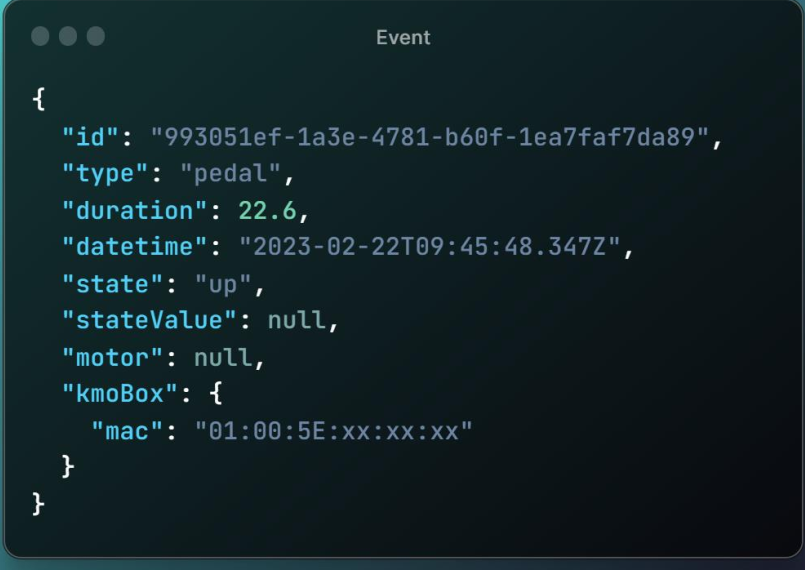
\includegraphics[width=10cm]{img/exemple_event.png}
    \caption{Exemple d'évênement renvoyer par les caisses}
    \label{fig:enter-label}
\end{figure}


\justify
\text En conclusion les bases de données sous le format SQL apportais plus d'avantage pour le projet et sont plus adaptée à notre utilisation de la base de donnée que les base de données noSQL.Nous avons donc choisie de les priviliégiés.  

\subsection{Connexion entre l'API WEB et les caisses}

\justify
\text Afin de de pouvoir connecter notre application web et  le système IOT qui récupère les différentes données remontées par les caisses .Un évênement est un Objets json qui est envoyé par la caisse sa structure est presque toujours la même et il concerne l'état d'un élement de la caisse (moteur,tapis etc ...) . Les évênements renvoyé peuvent aussi concerner  l'état de  la "gateway"(envoie des évênement au server web) comme l'état du boitier de commande de la caisse (création des évênements) et informe sur la température du cpu , tension...  afin de bien verifier que notre système n'ai pas de défaillance et faire de la maintenance à distance. Les caisses transmettent les événements par le biais de la "gateway" (en utilisant le protocole BLE), qui les envoie à son tour à l'API web. Pour réaliser cette dernière étape, il a fallu mettre en place un protocole de communication robuste c'est a dire qui doit pouvoir comuniquer une grande quantité de donnée au server web :  

\justify
\text Websocket est un protocole de communication server - client qui permet une communication bidirectionnelle persistante entre plusieurs clients et un serveur. Cela signifie que le serveur peut envoyer des données au client à tout moment, et vice versa, sans avoir besoin de renégocier les paramètres de la connexion à chaque requête. WebSocket permet une communication en temps réel, ce qui signifie que les données peuvent être transmises rapidement entre le client et le serveur. Cela est particulièrement utile pour les applications qui nécessitent une mise à jour rapide des informations. Ce protocole réduit la latence en établissant une connexion persistante entre le client et le serveur. Cela élimine le besoin de créer une nouvelle connexion à chaque demande, ce qui permet des échanges de données plus rapides.Il utilise une connexion unique pour gérer plusieurs échanges de données, ce qui réduit la surcharge du réseau et les ressources nécessaires par rapport à des méthodes traditionnelles comme les requêtes fréquentes.Mais cela implique aussi  d'introduire une couche de complexité supplémentaire dans le développement des applications web. La gestion des connexions, des erreurs, etc., nécessite une attention particulière pour garantir un fonctionnement fiable de l'application.

\justify
\text MQTT (Message Queuing Telemetry Transport)\footnote{Transport de Télémétrie à File d'Attente} est un protocole de messagerie léger et basé sur le modèle de publication/abonnement c'est a dire que un émetteur ouvre un flux de données sur lequel il met régulièrement à disposition des données , plusieurs clients peuvent s'abonner à ce flux, c'est-à-dire demander à être notifié dès qu'un nouveau message est publié . Il  est conçu pour être léger, ce qui signifie qu'il nécessite peu de ressources en termes de bande passante et de puissance de calcul. Il est efficace pour les appareils à faible puissance tels que les capteurs, les dispositifs IoT. MQTT est conçu pour minimiser la latence en permettant une communication asynchrone et il est ce protocole optimisé pour les échanges en temp réel.Il prend en charge des fonctionnalités telles que la reconnexion automatique. tous comme Websocket Mqtt comporte des inconvénients. Comparé à d'autres protocoles plus simples, la mise en œuvre de MQTT peut être plus complexe.MQTT nécessite un serveur intermédiaire qui reçoit, stocke et achemine les messages entre les clients MQTT. centralisé pour faciliter la communication entre les appareils. Cela peut ajouter une complexité supplémentaire à l'architecture de l'application. 

\justify
\text HTP(Hypertext Transfer Protocol)\footnote{Protocole de transfert hypertexte} est protocole courremant utiliser dans les applications webs nous l'avons directement juger hors propos car HTTP est exclusivement un protocole de communication unidirectionnelle, où le client doit envoyer une requête pour obtenir une réponse du server.Étant donné que ce procédé se traduit par un nombre conséquent de requêtes, cela peut entraîner une surcharge du réseau et une utilisation inéfficace de la bande passante. Le server  devant récepetionner plusieur millier de requête par seconde il s'ensuit HTTP n'est pas le protocole le plus adapté à nos besoins. 

\justify
\text Notre application nécessite une communication bidirectionnelle en temps réel, WebSocket est un bon choix. Il permet une communication instantanée entre le client et le serveur. Comparé à MQTT, WebSocket peut être plus simple à mettre en œuvre, surtout si on est  déjà familier avec les technologies web. WebSocket utilise des langages de programmation couramment utilisés pour le développement web, tels que JavaScript.



\vspace{20pt}

\centering
\begin{figure}[h]
    \centering
     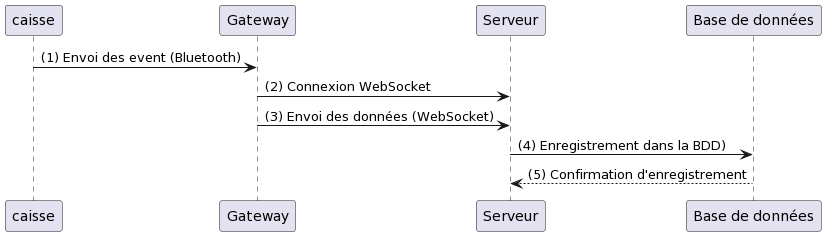
\includegraphics[width=\textwidth]{img/umlsequenceCheminEvent.png}
    \caption{Diagramme de séquence décrivant la génération, la transmission et la  sauvegarde des évênements}
    \label{fig:enter-label}
\end{figure}



\newpage
\justify
\subsection{Utiliser les données provenant des caisses }

\justify
\text Après avoir stocker de façon persistante les donnée et d'avoir définis un protocole de communication afin de pour réceptionner ces donnée je vais parler dans cette partie du document de la manière dont sont les données collectées dans l'application . 

\justify
\text Les évênement sont collecter dans le but est de permettre à un Algorithme de  définir si:
\begin{itemize}
    \item[$\bullet$] Elle nécessite urgemment une intervention. Cet état correspond à la situation où la caisse est déjà arrêtée pour cause de panne (ou encore fonctionnelle tout en présentant un risque élevé de tomber en panne de façon imminente). On parle de "maintenance urgente".La caisse présente alors des défauts majeur mais  le projet ne stoppera jamais la caisse logicielement .
    \item[$\bullet$]nécessite une opération de maintenance, sans pour autant que cette dernière ne revête un caractère urgent. On parle de "maintenance prédictive".La caisse présente alors des défaut mineurs
    \item[$\bullet$] La caisse est en état de fonctionnement normal, elle ne présente aucun défaut ni majeur ni minueur elle est soit récente  ou à eu une maintenance à été effectué récement.
\end{itemize}

\begin{figure}[H]
    \centering
    \includegraphics[width=\textwidth]{img/schéma_caisse.drawio (3).png}
    \caption{schéma des zone d'analys de la caisse par KMO-Predict}
    \label{fig:enter-label}
\end{figure}

\justify
\text Vous pouvez observer sur ce schéma les différentes parties de la caisse que KMO-Predict analyse.En numéro un, vous avez les cellules qui permettent au tapis d'avancer et de s'arrêter lorsque qu'un article passe devant. En numéro deux, il y a le capteur chargé de surveiller si la trappe s'ouvre (une sécurité qui coupe le moteur du tapis ). En numéro trois, vous avez le moteur du tapis, qui contient également le condensateur.Le numéros 4 est la pédale , la pédale permet de forcer l'activation du moteur du tapis de la caisse. La dernière flèche représente le boîtier KMO, qui relie la caisse aux différents projets regroupés par KMO, notamment dans KMO-Predict. Il permet l'envoi des données de la caisse , mais surtout il permet le contrôle et la gestion de la caisse.
\justify
\text Pour réaliser cette tâche j'ai du définir les différentes manière dont une caisse tombe en panne. Plusieur point que devra analyser l'algorithme on été soulevée grâce à l'experience ed COP-AMACO qui construit des caisses et fais du SAV dessus depuis de nombreuse année. Ils définiront l'état de maintenance de la caisse à des niveau plus ou moins critique : 

\vspace{12pt}
\begin{description}


    \item[Défaillance mineur:]   
        \begin{itemize}     
            \item[~]             
            \item[$\bullet$] La cellule (cf figure 6 n°3) permet au tapis d'avancer automatiquement, facilitant ainsi la mise à disposition des articles à scanner pour la caissière. Si nous constatons que la cellule ne donne aucun événement alors que la caisse est allumée, cela entraîne un défaut mineur de la caisse. L'algorithme détermine alors l'état de la caisse comme étant en maintenance "prédictive".
            
            \item[$\bullet$]Activation de la trappe (cf figure 6 n°1) durant 3 jours : la trappe est munie d'un capteur elle est une  sécurité, elle peut parfois s'ouvrir toute seule et ainsi arrêter le tapis. La cause de ce défaut est le plus souvent un encrassement du tapis, mais nous examinerons attentivement pendant 3 jours avant de mettre la caisse en maintenance "prédictive", afin de ne pas prendre en compte les ouvertures de trappes nécessaires à la sécurité des clients. Cela n'empêche en aucun cas la caisse de fonctionner et est donc considéré comme un défaut mineur.
            
            \item[$\bullet$] Utilisation fréquente de la pédale (cf figure 6 n°4 ) pendant 7 jours consécutifs : la pédale sur une caisse permet de forcer l'activation du tapis lorsque les capteurs sensés faire avancer le tapis sont en panne temporaire. Elle fonctionne ainsi jusqu'à ce que des articles passent devant et que l'activation du tapis devienne automatique. Si nous constatons une utilisation trop fréquente de la pédale, cela peut indiquer un dysfonctionnement des capteurs ou un autre problème avec le tapis de la caisse. L'algorithme considérera cela comme un défaut mineur et définira l'état de maintenance de la caisse en "prédictive".
            
             \item[$\bullet$] La caisse n'a pas été allumée depuis 3 mois ou n'a renvoyé aucun événement depuis 3 mois. Cela peut signifier que la caisse est en panne et n'a donc jamais été allumée (défaut non pris en compte dans l'algorithme). Cela peut également indiquer une défaillance dans le système IOT de KMO-PREDICT, comme une panne de la gateway ou des KMO-Box (les boîtiers dans la caisse qui renvoient les événements à la gateway). Dans ce cas, l'algorithme définira l'état de maintenance en "prédictive" pour signaler aux utilisateurs que la caisse présente peut-être un souci.
             
              \item[$\bullet$] La date d'installation est supérieur à 2 ans. Une caisse qui à plus de 2 ans d'installation si elle n'est pas réviser assez souvent à tendance à tomber en panne pour évité un défaut majeur sur la caisse l'algorithme définira l'état de la caisse en maintenance "prédictive" afin de signaler à l'utilisateur de faire réviser la caisse. 
        \end{itemize}

         
    
\end{description}

\begin{description}
    \item [Defaillance majeur ]
        \begin{itemize}
           \item[~]
            \item[$\bullet$] La caisse a plus de 8000 heures de fonctionnement. L'entreprise COP-AMACO sait que le condensateur dans le moteur de la caisse se casse au bout d'environ 8000 heures de fonctionnement. Il est donc possible d'analyser le temps de fonctionnement de la caisse. Si ce dernier atteint les 8000 heures, la caisse sera presque certainement stoppée. Une approche à plus ou moins 1000 heures des 8000 heures de fonctionnement entraînera une maintenance préventive, tandis qu'une fois les 8000 heures atteintes, cela passera l'état de maintenance de la caisse en maintenance urgente.
            
            \item[$\bullet$] Vérifiez si le capteur thermique du moteur de la caisse ne se déclenche pas. Si le capteur thermique du moteur se déclenche, cela peut provenir de problèmes concernant le tapis de la caisse, qui risque à force d'endommager le moteur. Ce défaut est considéré comme un défaut majeur de la caisse. L'algorithme définira alors l'état de la caisse en maintenance urgente, car cela peut causer des dégâts importants au moteur.
        \end{itemize}
\end{description}



\begin{figure}[H]
    \centering
    \includegraphics[width=\textwidth,height = 20cm]{img/Schéma_algoryhtme.pdf}
    \caption{Schéma simplifier de la fonction Lambda}
    \label{fig:enter-label}
\end{figure}

\justify
\text Dans le graphique ci-dessus, vous pouvez observer une simplification de l'algorithme. J'ai regroupé les pannes en 2 catégories : les défaillances mineures qui représentent un risque pour la caisse de tomber en panne, mais qui lui permettent encore de fonctionner, et les risques majeurs qui sont des risques pouvant détruire la caisse, nécessitant une réparation urgente, ou entraîner un arrêt complet de la caisse, exigeant la venue d'un technicien en urgence.Ce schéma illustre les quatre cas que la fonction lambda va détecter. Cet algorithme permettra de définir le niveau de maintenance de la caisse, qu'il soit en état de fonctionnement, nécessitant une maintenance préventive ou une maintenance urgente. Nous pouvons constater que la détection d'un défaut mineur entraînera dans tous les cas une mise en maintenance urgente de la caisse afin de prévenir notre client et de lui signaler qu'il doit arrêter l'exploitation de cette caisse.Ensuite, le code va créer un tableau avec la MAC de la caisse, ainsi que tous les défauts détectés et le niveau de maintenance défini, puis l'envoyer à l'API de KMO-PREDICT.

\justify
\text Afin de développer l'algorithme de maintenance prédictive, nous devons prendre en compte plusieurs éléments, tels que la fréquence d'exécution, le langage utilisé et l'architecture pour optimiser ses performances. Différentes options s'offrent à nous :

\begin{itemize}
    \item[$\bullet$] Intégrer l'algorithme dans l'API de KMO-predict.
    \item[$\bullet$] Ajouter un conteneur Docker sur le serveur pour séparer l'algorithme du reste de l'application.
    \item[$\bullet$] Héberger l'algorithme sur un autre serveur pour ne pas ralentir les applications en cours sur le serveur de production, notamment en cas de demandes d'analyses fréquentes et lourdes.
    
\end{itemize}
\text La solution retenue est la troisième, car elle offre une meilleure scalabilité \footnote{La scalabilité fait référence a la capacité d’un système, d’une application ou d’une infrastructure a s’adapter et a gérer efficacement une augmentation de la charge de travail ou du nombre d’utilisateurs} de l'application.

\justify
\text Maintenant, expliquons pourquoi nous avons choisi d'utiliser AWS Lambda. AWS Lambda est un service de calcul sans serveur qui nous permet d'exécuter du code sans avoir à gérer les serveurs sous-jacents. Les principales raisons pour lesquelles nous avons opté pour AWS Lambda sont les suivantes :

\begin{itemize}
    \item[$\bullet$]  AWS Lambda permet de gérer automatiquement la montée en charge et la réparti\-tion de la charge. Ainsi, si la demande d'analyses augmente, Lambda s'adapte automatiquement pour fournir les ressources nécessaires.

    \item[$\bullet$]  En utilisant AWS Lambda, nous n'avons pas à nous soucier de la configuration et de la gestion d'un serveur. Tout est pris en charge par AWS, ce qui réduit la complexité et les responsabilités opérationnelles.

    \item[$\bullet$]  AWS Lambda, nous ne payons que pour le temps d'exécution réel de notre code, ce qui permet d'optimiser les coûts. Si l'algorithme de maintenance prédictive n'est pas utilisé en permanence, nous ne payons que lorsque des analyses sont effectuées.
\end{itemize}


\justify
\text L'algorythme prend en entrée un tableaux d'évênement présenté en amont dans ce document (cf figure 4 )  afin de produire un rapport d'état des caisses (cf figure 8) qui contient l'adresse MAC du boitier de la caisse , l'état prédit par l'alogrithme ainsi que une liste des erreur majeur ou mineur que le programme à détectée le cas échéant . 
\justify

\centering
\begin{figure}[H]
    \centering
    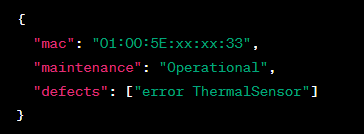
\includegraphics[width=10cm]{img/json-report.png.png}
    \caption{Exemple de rapport de l'algorithme de aws lambda}
    \label{fig:enter-label}
\end{figure}


\justify
\text Grâce à ce processus nous somme maintenant capable de détecter si une caisses est en panne ou non ainsi que l'élément qui lui ferais défaut. Dans la prochaine partie je parlerais des dévellopement efféctué coter front end de l'applications et comment est son présenté le résultat de l'algorythme aux différents utilisateur.

\subsection{Afficher les résultat de l'algorithme}

\justify
\text Pour présenter les résultats de l'algorithme de prédiction et permettre aux futurs utilisateurs de les exploiter, nous avons développé une interface utilisateur (IHM). Dans le domaine du développement web, il existe plusieurs frameworks populaires tels que Angular, React et Vue. Chaque framework présente ses propres avantages. Nous avons opté pour le framework Angular afin de maintenir une cohérence avec la direction de nos produits digitaux chez COP-AMACO. Angular présente l'avantage de créer des applications à page unique, ce qui signifie que l'application ne charge que une seule fois la structure et ne nécessite pas de rechargement de page , avec Angular seule les données sont échanger. Ainsi, nous avons choisi d'utiliser Angular pour notre IHM, afin d'offrir une expérience utilisateur fluide et rapide.  

\justify
\text L'interface utilisateur sera conçue de manière simple et intuitive, avec une liste de grands boutons représentant les différentes caisses. Chaque bouton sera accompagné d'un logo indiquant l'état de la caisse. L'objectif principal est de permettre à l'utilisateur de visualiser rapidement l'état de maintenance de chaque caisse.
Si une caisse est en maintenance prédictive, un petit icône jaune sera affiché à côté du bouton correspondant, indiquant ainsi à l'utilisateur qu'une maintenance préventive est recommandée. Cela permettra de signaler qu'il pourrait être judicieux de planifier une révision pour éviter tout défaut potentiel.
D'autre part, si une caisse est en maintenance urgente, un petit icône rouge sera affiché à côté du bouton correspondant, alertant ainsi l'utilisateur qu'une intervention immédiate est nécessaire pour résoudre un problème critique. Cela permettra d'attirer l'attention de l'utilisateur sur les caisses qui nécessitent une action rapide.
L'objectif global de cette interface est de fournir une visualisation claire et concise de l'état de maintenance de chaque caisse, permettant ainsi à l'utilisateur de comprendre rapidement et facilement si des actions sont requises pour maintenir le bon fonctionnement des caisses.


\centering
\begin{figure}[H]
    \centering
    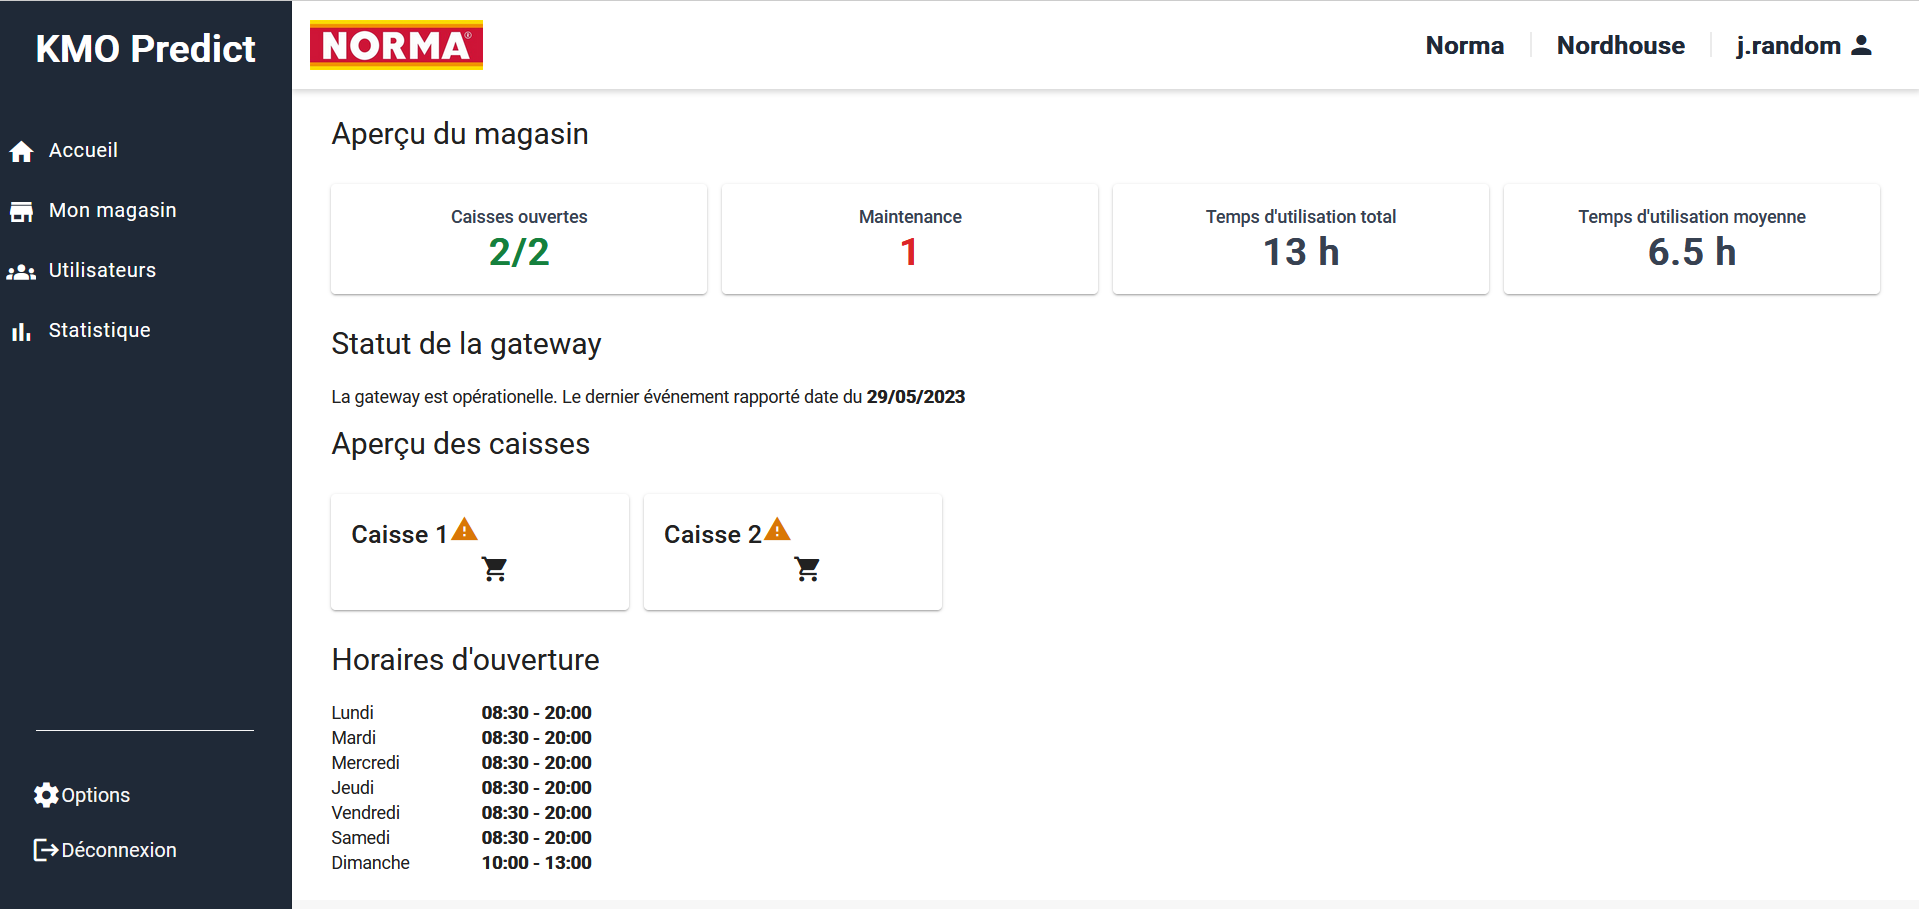
\includegraphics[width=\textwidth]{img/interface_client_predict.png}
    \caption{Interface client de KMO Predict}
    \label{fig:enter-label}
\end{figure}
 

\justify
 \text Nous avons également veillé à ce que l'utilisateur client de COP-AMACO puisse accéder à des informations plus précises concernant l'état de la caisse, ainsi que des statistiques détaillées sur son utilisation, telles que la durée d'utilisation, le nombre de clients passés par caisse et les messages d'erreur renvoyés par l'algorithme de maintenance prédictive.

 \justify
 \text L'application a deux objectifs principaux. Tout d'abord, elle permet aux gestionnaires de magasin de connaître le niveau de maintenance de leur parc de caisses. Ensuite, elle aide l'équipe du service après-vente de COP-AMACO à détecter les pannes potentielles ou avérées des caisses de tous les clients, afin de proposer des interventions anticipées.Cette interface joue également un rôle crucial en vérifiant la connexion de la partie IoT du projet KMO-PREDICT. Si la connexion est interrompue, cela peut empêcher le projet de fonctionner correctement, car il ne reçoit pas de nouvelles données. De plus, l'application peut analyser les magasins les plus à risque, tels que ceux où de nombreuses caisses sont en maintenance préventive, ainsi que les magasins nécessitant un traitement urgent où la plupart des caisses sont en panne.

 \justify
 \text Nous avons développé une interface  spécialement pour les utilisateurs de l'application, qui sont des membres de COP-AMACO chargés d'assurer le bon fonctionnement de l'application et la surveillance complète du parc de caisses. Dans cette partie de l'application, nous leur présentons une liste des clients possédant des caisses connectées. Des filtres ont été mis en place du côté de l'API afin de garantir un un haut niveaux de performance de l'interface utilisateur.Nous avons du mettre des outils de filtrages et de pagination efficace(back-end et front-end car COP-AMACO pourrais être amenée à surveiller plusieur milliers de caisse avec ce système et cela pourrais amméner des pertes significative de performances. Les utilisateurs ont un accès permanent aux magasins présentant le plus de caisse en maintenance urgente et préventive, ainsi qu'à la liste des magasins actuellement déconnectés mais équipés du module KMO-PREDICT. L'interface a été conçue pour être la plus intuitive possible. Lorsque l'utilisateur clique sur un client dans la liste des magasins, il peut accéder aux informations spécifiques à la ligne de caisses de ce client, y compris l'état de maintenance de chaque caisse.


\centering
\begin{figure}[H]
    \centering
   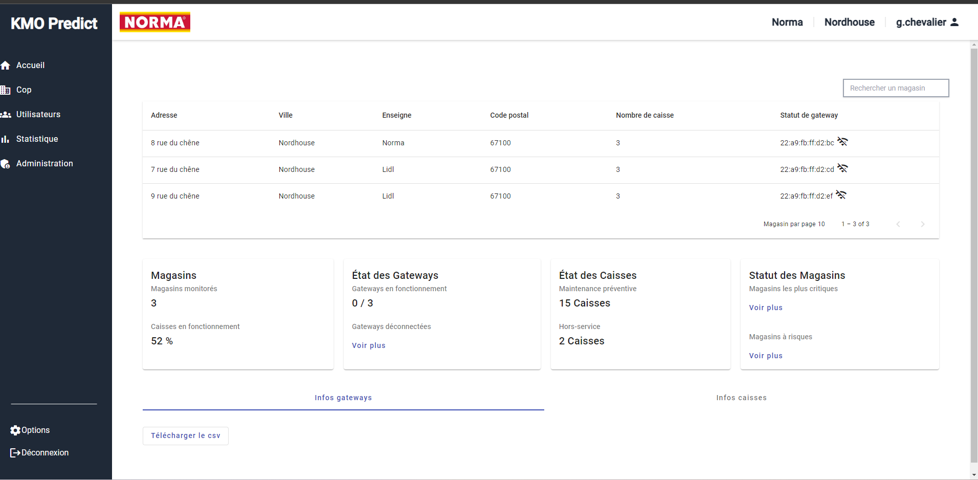
\includegraphics[width=\textwidth]{img/interace_admin.png}
    \caption{Interface de gestion par COP  de KMO Predict}
    \label{fig:enter-label}
\end{figure}
 
 \justify
 \text Tout comme le client, l'utilisateur de COP-AMACO a accès à des informations plus détail\-lées sur les caisses, bien que différentes de celles du client. Évidemment, il n'est pas intéressé par les calculs de rendement de la caisse. Cependant, il dispose de données plus approfondies, telles que les informations concernant la carte électronique de la caisse (Température du CPU,version du firmware, etc.). De plus, il a accès à des données telles que la date de la dernière maintenance, la date d'installation des caisses et le journal des erreurs.Ces informations permettent aux managers des techniciens de cibler plus facilement les tâches à effectuer sur site et de les communiquer aux techniciens chargés de réparer la caisse.

\begin{figure}[H]
    \centering
    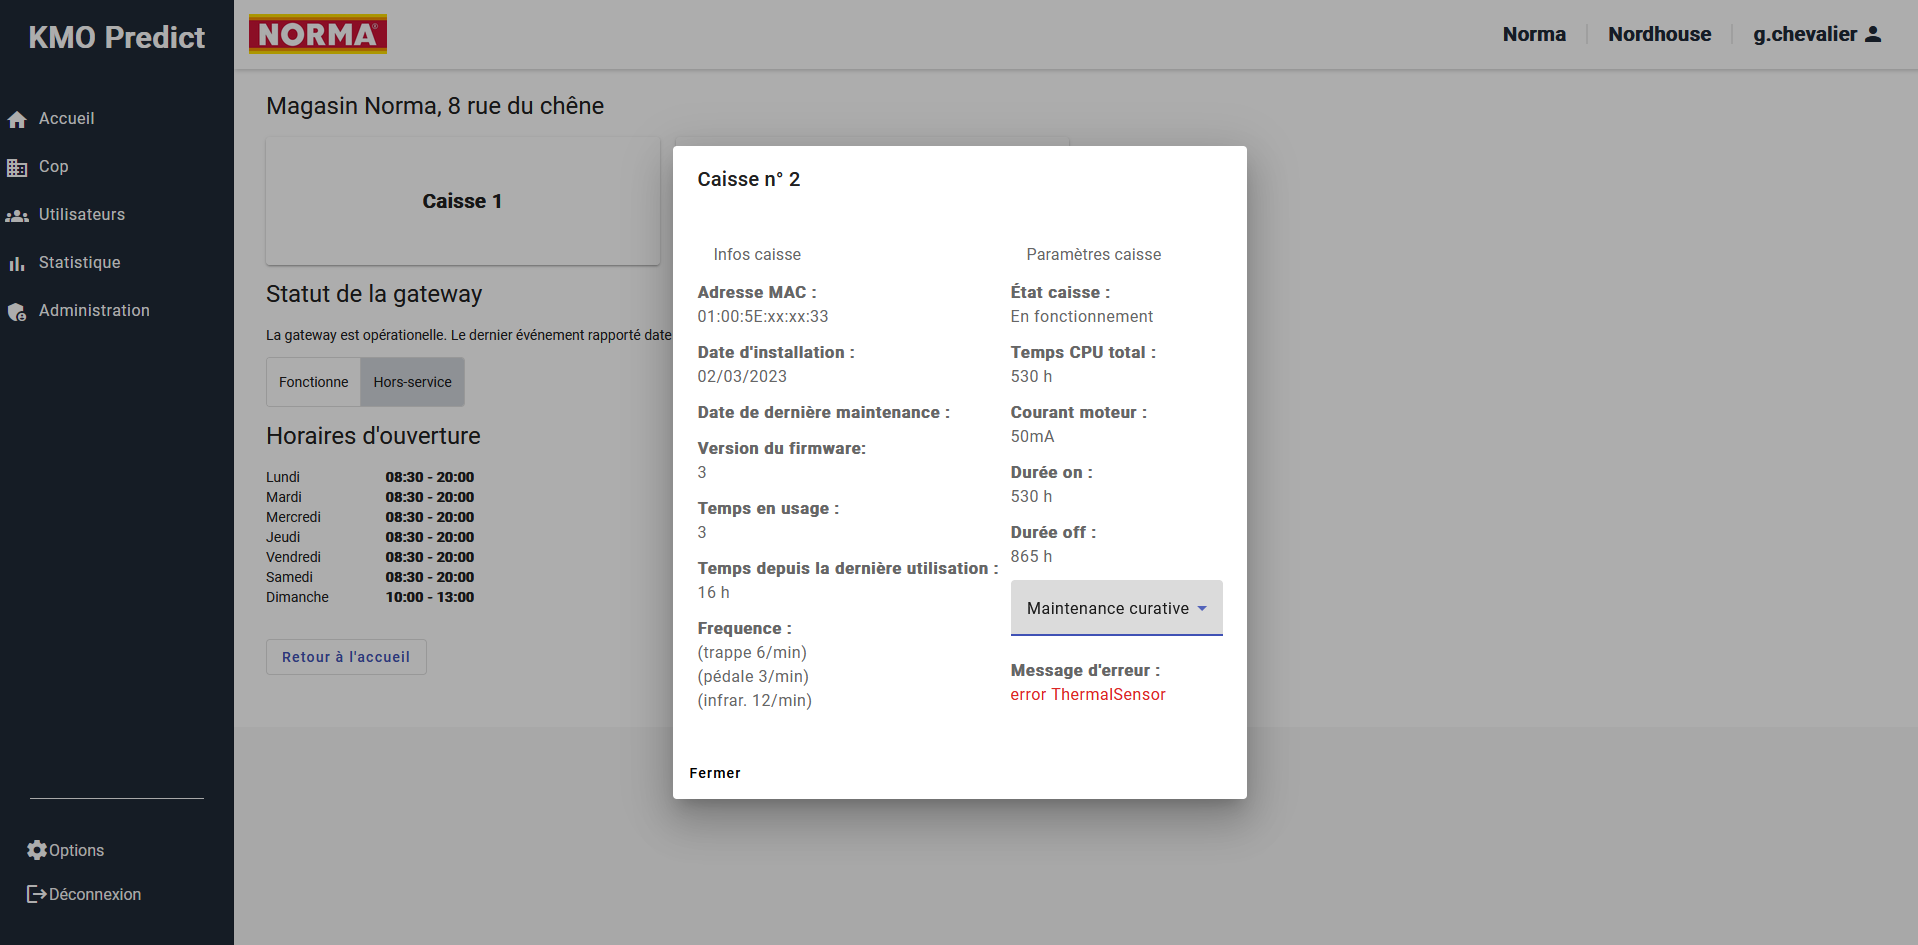
\includegraphics[width=\textwidth]{img/VIEW_cop_admin.png}
    \caption{Interface détailler d'une caisse pour l'administrateur}
    \label{fig:enter-label}
\end{figure}

 \subsection{Interface de gestion du système IoT et des magasins }

\justify
\text Nous avons précédemment développé deux interfaces principales qui sont au cœur de notre projet. Ces interfaces montre la fonctionnalité principale de notre application, à savoir la gestion des lignes de caisses. Toutefois, il persistait un problème à surmonter. En effet, notre projet dépend largement de la communication entre des cartes électroniques physiques. Celles-ci peuvent parfois nécessiter un remplacement en raison d'une panne ou d'un défaut. Pour résoudre ce problème, nous avons créé une interface de gestion des magasins et des gateways. Une gateway est une carte qui fait le lien entre le web et les cartes des différentes caisses des magasins.Ainsi, nous avions besoin de créer une interface spécifique pour la gestion du projet. Cette interface nous permet de changer l'adresse MAC de la gateway qui lie dans la base de donnée un magasin à sa gateway. De plus, cette interface vise également à permettre à l'utilisateur de mettre à jour les données des magasins.

\justify
\text Pour concevoir cette partie de l'application, il nous a fallu porter notre réflexion sur l'avenir de cette dernière. Anticiper les éventuelles difficultés techniques qu'elle pourrait rencontrer a été un élément essentiel de notre processus. Plus important encore, nous avons dû envisager des solutions simples, efficaces et aisément accessibles pour remédier à ces problèmes.

\justify
\text Nous souhaitions que notre application soit simple à comprendre et surtout qu'elle reste sur une seule page afin d'éviter de désorienter l'utilisateur. Pour ce faire, nous avons employé des fenêtres contextuelles (créées avec Angular Material). . Elles permettent d'intégrer facilement différentes fonctionnalités qui, autrement, pourraient nécessiter l'ajout d'une nouvelle page, tout en restant sur la page en cours. Ces boîtes de dialogue offrent un design moderne et une grande personnalisation. De plus, elles  intègrent des animations et gèrent les superpositions. En somme, leur intégration facile et leur polyvalence font de ces fenêtres contextuelles un outil précieux pour maintenir une interface utilisateur claire et efficace.

\begin{figure}[h]
    \centering
    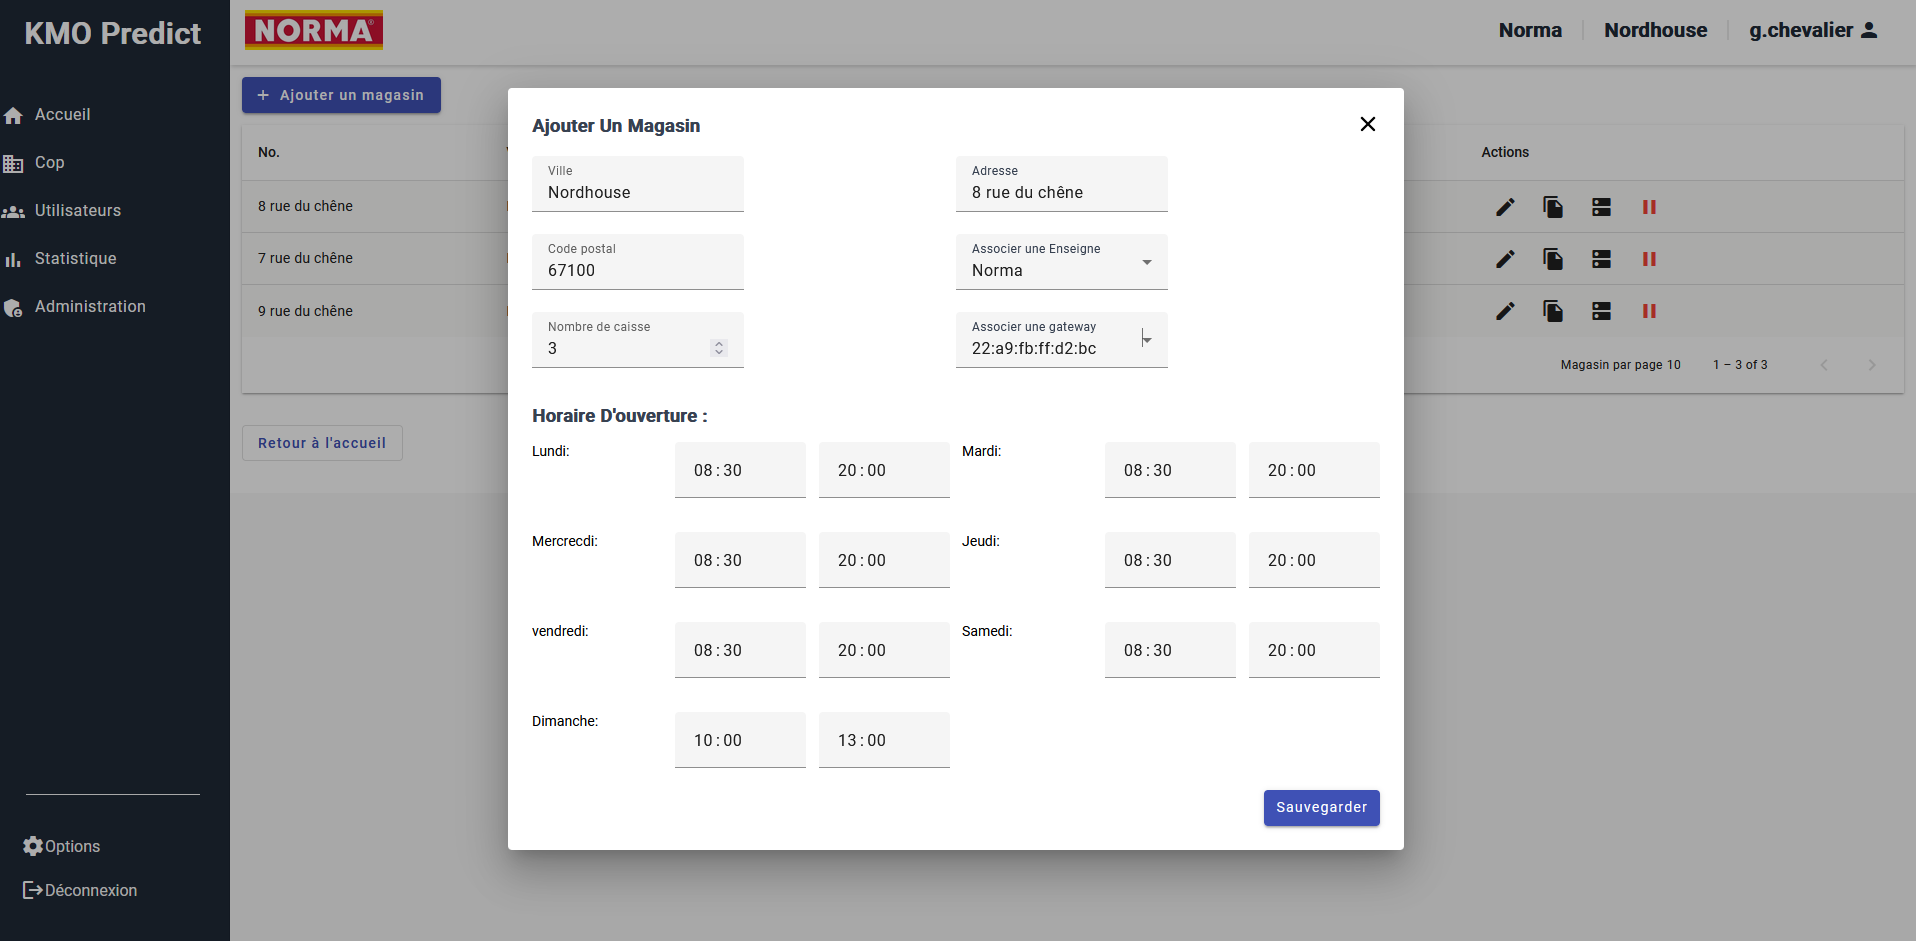
\includegraphics[width=\textwidth]{img/interface_admin_update_mag.png}
    \caption{PopUp de gestion des informations du magasin}
    \label{fig:enter-label}
\end{figure}

\justify
\text Comme illustré sur l'image ci-dessus, l'administrateur de l'application a la capacité de modifier diverses informations relatives au magasin, y compris sa "Gateway", en cas de remplacement par un technicien de l'entreprise. Vous pouvez remarquer, en arrière-plan, différentes icônes qui autorisent l'utilisateur à exécuter certaines actions sur les magasins. 


\justify
\text L'icône en forme de crayon active la fenêtre contextuelle visible sur l'image. L'icône à coté donne la possibilité de dupliquer un magasin. L'objectif n'est pas de créer un simple doublon, mais plutôt de faciliter l'ajout de nouveaux magasins appartenant à la même enseigne, dont les informations sont généralement très similaires. Cela permet à l'administrateur de créer un nouveau magasin sans avoir à remplir tous les champs à nouveau : il lui suffit de modifier les informations qui diffèrent.

\justify
\text C'est précisément dans ce genre de situation que l'utilisation d'Angular révèle toute son utilité. Au lieu de concevoir une fenêtre contextuelle distincte pour chaque utilisation nécessitant les mêmes champs, nous pouvons réutiliser le code de la fenêtre qui sert à l'ajout des magasins pour la mise à jour et la duplication de ceux-ci. Pour cela, j'ai créé un composant Angular qui, en fonction du bouton sélectionné, permet de mettre à jour, d'ajouter ou de dupliquer un magasin. Mais pour l'utilisateur, cette complexité reste invisible, ce qui nous évite de coder plusieurs fois la même interface. Cela représente un gain de temps considérable dans le développement de ce genre de fonctionnalité, et illustre parfaitement l'intérêt d'utiliser Angular.

\subsection{Tester unitairement l'application début d'une CI \textbackslash CD}

\justify
\text 
Dans le but de limiter le risque de régression, à la moindre addition de code, nous avons mis en place une pratique qui consiste à tester les différentes fonctions que nous créons. Cela permet de vérifier que chaque modification ultérieure de ces dernières n'entraîne pas de régression dans l'application. Dans un premier temps, nous verrons ce qu'est un test unitaire. Ensuite, nous examinerons comment et quand nous utilisons les tests unitaires pour éviter les régressions potentielles.

\justify
\text Les tests unitaires sont une pratique de développement  qui consiste à évaluer individuellement les composants d'un programme de manière à s'assurer qu'ils fonctionnent correctement et qu'ils produisent les résultats attendus. Ces tests sont effectués sur des petites parties de code, qui peuvent être des fonctions, des méthodes ou même des classes.Le principal objectif des tests unitaires est de détecter les erreurs et les bugs dans les parties du code testées. Ils permettent aux développeurs de valider le bon fonctionnement de chaque unité de manière isolée, ce qui facilite grandement la détection et la résolution des problèmes. De plus, les tests unitaires rendent le code plus fiable, maintenable et évolutif, car ils permettent de repérer rapidement les régressions lorsqu'on apporte des modifications au code existant.

\justify
\text Lorsqu'on écrit des tests unitaires, on essaie de couvrir différents scénarios pour chaque bout de code testé. Cela inclut les cas où les entrées sont valides, les cas où elles sont incorrectes, ainsi que les cas limites et les cas d'erreur. L'objectif est d'obtenir une couverture de test élevée pour s'assurer que toutes les branches et les comportements du code sont correctement vérifiés. La couverture des tests dans le code d'un projet est exprimée en pourcentage appelé le "coverage".La couverture de test mesure le pourcentage de code exécuté lors de l'exécution des tests par rapport au code total du projet. Un taux élevé de couverture de test signifie qu'une grande partie du code est testée, ce qui augmente la confiance dans la robustesse et la fiabilité de l'application web. Cependant, une couverture élevée ne garantit pas que tous les bugs ont été trouvés. Il est, en pratique, impossible de couvrir tous les scénarios possible: il y a souvent beaucoup trop de cas à tester.

\justify
\text Pour les tests liés au projet, nous avons convenu qu'un taux de couverture de code d'environ 80\% serait satisfaisant. Étant donné que nous utilisons NestJS et Angular des frameworks pour de NodeJS, qui repose sur de nombreuses bibliothèques tierces, nous avons décidé de ne pas tester certaines parties du code pour gagner du temps pourtant les nodes modules étant fait par la communauté , en cas de mise à jour de ces dernières certaine nouvelle version pourrais créer des failles dans l'application. Nous avons estimé que le code coverage équivalent au non-test de ces modules Node représenterait 20\% de couverture de code, ce qui est légèrement inférieur à l'objectif initial.

\justify
\text Afin de tester l'application, nous avons choisie un framework dédié aux tests unitaires pour facilité la rédaction de ces derniers.Parmis les nombreux framework de test disponible nous nous sommes tournée vers jest pour différente raison : 
\begin{itemize}
    \item[$\bullet$] Jest est réputé pour sa simplicité et sa facilité d'utilisation. Son interface intuitive permet aux développeurs de définir facilement des cas de test, d'exécuter des suites de test et d'interpréter les résultats sans effort supplémentaire.
    \item[$\bullet$]  NestJS et Angular sont souvent utilisés avec TypeScript pour bénéficier des avantages du typage statique. Jest offre une prise en charge native de TypeScript, permettant aux développeurs d'écrire des tests en TypeScript et de tirer parti des vérifications de type pour une meilleure qualité du code.
    \item[$\bullet$] Par défaut, Jest exécute les tests en parrallèle. Cela permet de gagner du temps  lors de l'exécution de suites de tests volumineuses, ce qui est le cas pour les projets de grande envergure.
    \item[$\bullet$] Jest offre une gamme complète d'outils pour simuler des requêtes HTTP, des bases de données et d'autres dépendances externes. Cela simplifie le test des fonctionnalités complexes tout en maintenant un contrôle total sur l'environnement de test.
    \item[$\bullet$] Jest bénéficie d'une communauté active, avec un support continu et une évolution régulière.
\end{itemize}
\justify
\text Dans le but de simplifier les tests de l'application dans sa globalité, nous avons choisi d'utiliser Jest pour tester à la fois le back-end et le front-end. Jest est déjà intégré dans NestJS, mais pour Angular, il nécessite une installation séparée, contrairement au framework Karma qui est intégré nativement pour les tests.Cependant, nous avons décidé de ne pas utiliser Karma pour plusieurs raisons:
\begin{itemize}
    \item[$\bullet$] La configuration initiale de Karma peut être complexe, en particulier pour les nouveaux utilisateurs. Il nécessite souvent la mise en place de fichiers de configuration et de plugins supplémentaires
    \item[$\bullet$]  En raison de sa complexité, Karma peut avoir une courbe d'apprentissage plus lente que celle de Jest.
    \item[$\bullet$] Les tests exécutés via Karma peuvent prendre plus de temps, en particulier dans des projets volumineux, ce qui peut ralentir le processus de développement et de test.
    \item[$\bullet$]  Karma s'appuie sur de vrais navigateurs ou des navigateurs virtuels pour exécuter les tests. Cela signifie que les tests peuvent varier en fonction du navigateur utilisé, ce qui peut entraîner des incohérences entre les résultats des tests sur différents navigateurs.
    \item[$\bullet$] Bien que Karma dispose d'une documentation fournie, certains aspects du framework peuvent manquer de détails ou de clarté, ce qui peut rendre la résolution de problèmes plus difficile. 
    \item[$\bullet$] Nous préférons centraliser tous nos tests au sein de Jest pour une plus grande cohérence et une gestion simplifiée des tests sur les deux parties de l'application. Cela nous permettra également d'exploiter pleinement les fonctionnalités de Jest, telles que le mocking, les assertions avancées, et les performances accrues qu'il offre.


\end{itemize}
\justify
\text Dans l'API de l'application, nous effectuons des tests sur l'ensemble des différentes méthodes que nous développons. Nous vérifions que chaque fonction existe bien et qu'elle renvoie des données cohérentes. L'objectif de ces tests est de s'assurer que les données communiquées par l'API ne divergent pas de ce qui est attendu dans la partie frontend, ainsi que dans les communications avec le système IOT via le serveur de websocket. Nous vérifions également que le websocket est bien instancié et qu'il répond correctement aux différents événements auxquels il doit réagir.

\justify
\text Dans la partie frontend, nous effectuons des tests sur les différents composants pour vérifier qu'ils sont correctement définis. Nous vérifions également les fonctions pour nous assurer qu'elles existent et qu'elles renvoient les résultats attendus si elles sont liées à une partie du code dans l'interface. Nous vérifions que chaque bouton, qui est censé activer certaines fonctions, est bien présent et qu'il est correctement lié à la fonction correspondante. Cela nous permet de nous assurer que les fonctions n'ont pas été modifiées depuis la dernière vérification, afin d'éviter les bugs où une fonction ne se lance pas correctement.

\justify
 À ce stade du développement, les tests que nous avons effectués sont essentiellement des tests unitaires. Les tests d'intégration viendront par la suite, pendant que le temps de développement sera davantage axé sur l'ajout de nouvelles fonctionnalités.

\justify
\text Nous n'exécutons pas tous ces tests manuellement à chaque nouvelle fonctionnalité. Pour que notre application soit régulièrement testée, notamment à chaque nouvel ajout, nous avons mis en place une CI (Intégration Continue) sur notre dépôt Git. Cette CI permet d'exécuter les scénarios de test que nous avons définis à l'avance. Avant d'accepter chaque requête de fusion sur la branche "develop" de notre dépôt ,une branche importante pour nous, étant l'un des derniers maillons avant la mise à jour de la branche principale du dépôt (qui ne doit contenir que des versions fonctionnelles de l'application).

\begin{figure}[H]
    \centering
    \includegraphics[width=\textwidth]{img/CI_schéma.drawio.png}
    \caption{Les différente étapes du processus de la CI}
    \label{fig:enter-label}
\end{figure}

\justify
\text
Dans ce schéma, nous pouvons observer les différentes étapes réalisées par la CI (Intégration Continue). Tout d'abord, nous effectuons l'installation des dépendances pour les projets NestJS et Angular. Cela inclut le téléchargement de tous les modules nécessaires pour que les applications puissent être construites et fonctionner correctement. Ensuite, nous procédons à la vérification du code (linting). Cette étape permet de s'assurer que le code est au bon format, qu'il respecte les conventions définies dans le projet, et qu'il n'y a pas de log oubliés dans la console. Cela nous garantit un code de qualité tout au long du projet.La troisième étape consiste à compiler l'application afin de vérifier si elle démarre correctement. Cela nous permet de détecter d'éventuelles erreurs dans le code qui pourraient empêcher le bon fonctionnement de l'application lors de sa mise en production.Enfin, la quatrième étape concerne l'exécution des tests pour vérifier le comportement de l'application en fonction des scénarios de test écrits. Pour l'instant, nous nous concentrons sur la création de tests unitaires pour notre application. Cependant, plus tard dans le développement, nous envisageons de mettre en place des tests "end-to-end" (E2E) afin d'améliorer sa fiabilité.Le test end-to-end (E2E) est une approche de test qui vise à évaluer le fonctionnement complet d'une application ou d'un système en simulant les interactions d'un utilisateur réel avec l'ensemble du système, de bout en bout. L'objectif du test E2E est de vérifier que toutes les parties de l'application fonctionnent correctement ensemble et de valider le flux de travail complet, depuis le début jusqu'à la fin.Les tests E2E sont essentiels pour garantir que notre application est solide et fiable, car ils reproduisent les scénarios réels d'utilisation et peuvent détecter des problèmes qui pourraient échapper aux tests unitaires ou à d'autres formes de tests isolés. Nous reconnaissons que leur mise en œuvre peut être plus complexe et demander plus de ressources en termes de temps et d'efforts, mais ils seront bénéfiques pour assurer la qualité globale de l'application avant sa mise en production.

\justify
\text Notre dépôt Git est hébergé sur l'application web GitHub. Dans GitHub, la CI est appelée "Actions". Dans la section "Actions", vous retrouverez les différentes fois où votre CI a été exécutée, ainsi que les résultats et le temps qu'elle a mis pour s'exécuter. Pour configurer la CI dans GitHub et lui indiquer quand elle doit s'exécuter, ainsi que les actions à effectuer, notamment le lancement des tests, il faut créer un fichier selon cette architecture : ".github/workflows/ci.yml". Les instructions pour la CI s'écrivent dans le langage YAML (YAML Ain't Markup Language), qui est un langage de sérialisation de données utilisé pour représenter des informations structurées sous forme de texte. Une autre application du langage YAML serait la configuration d'un docker-compose. Le format YAML est souvent utilisé pour configurer des applications, stocker des données ou définir des documents lisibles par l'homme. Il est couramment utilisé dans des scénarios tels que la configuration de fichiers, la gestion de paramètres et l'échange de données entre applications.

\justify
\text En mettant en place des tests ainsi qu'une CI (Intégration Continue), nous assurons que le projet reste maintenable dans le temps, tout en détectant d'éventuelles régressions liées à l'ajout de nouvelles fonctionnalités. Actuellement, dans le processus de CI/CD, seule la partie CI a été développée, mais nous avons l'espoir d'ajouter la partie CD (Déploiement Continu) ultérieurement, une fois qu'une version Alpha aura été testée et déployée pour la première fois, et que nous aurons amélioré nos scénarios de test. Cette approche nous permettra de fournir aux utilisateurs, dans les meilleurs délais, les dernières fonctionnalités ajoutées par l'équipe de développement.


\newpage
\section{Conclusion}

\justify
\text
Mes trois années de formation à l'UHA 4.0 m'ont apporté les connaissances en développe-\ ment informatique nécessaires pour les appliquer au sein d'entreprises et d'associations. Pendant mes périodes de stage et d'alternance, elles ont décidé de me faire confiance et m'ont permis d'accroître mes connaissances dans le milieu du développement, ce qui a été bénéfique pour mon processus d'apprentissage. J'ai également pu participer au développement de divers projets qu'ils avaient à effectuer.
\justify
\text
Pendant mon cursus, j'ai eu la chance de rejoindre l'entreprise COP-amaco pour un contrat de professionnalisation d'une année, intégrant leur équipe chargée du développem-\ ent des services digitaux. J'ai travaillé sur divers projets dès leurs démarrages, ce qui m'a permis de participer à leur mise en place en accord avec les demandes des clients.
\justify
\text
Je suis convaincu d'avoir progressé d'un point de vue professionnel, technique et méthodo-\ logique. Sur le plan technique, j'ai mis en application ce que j'ai appris pendant ma formation à l'UHA 4.0 et j'ai également réussi à me former pour acquérir des compétences dans des technologies que je ne connaissais pas. Professionnellement, j'ai collaboré avec les autres membres de l'équipe de développement pour être efficace et réaliser les diverses fonctionnalités des applications qui m'ont été assignées, et j'ai parfois été force de proposition. En termes de méthodologie, j'ai réussi à utiliser les méthodes apprises en cours pour m'autoformer pendant mon apprentissage sur certaines technologies et sujets de gestion de projet.
\justify
\text
Dans ce document, j'ai présenté le projet KMO-Predict, auquel j'ai le plus contribué durant mon alternance. Débuté en fevrier, cette application est actuellement en phase de test dans nos locaux afin de vérifier tous les différents éléments qui la composent. Nous devons nous assurer que nos développements entre la partie web et IoT sont corrects et concordent pour qu'ils puissent communiquer ensemble. Au niveau du web, nous avons  développé la plupart des fonctionnalités du cahier des charges. L'application web permet d'accéder aux données des caisses pour les gestionnaires de magasin et COP.Le mécanisme permettant d'émettre et de transmettre les événements liés aux caisses est fonctionnel. Un algorithme permet de définir et de mettre à jour le niveau de maintenance d'une caisse. Un espace d'administration permet de gérer les magasins présents dans l'application ainsi que de faire la gestion des gateways.
\justify
\text
Le développement des fonctionnalités de la première version de l'application est presque achevé sur la partie web. Dans les futures versions de l'application, nous aimerions ajouter des accès à notre API afin de permettre à nos clients d'exporter les données des caisses avec leurs outils de BI (business intelligence). Nous souhaitons également rendre l'application compatible avec une utilisation sur tablette et smartphone, ainsi qu'ajouter une application ou un module dans l'application SAV que nous avons créée en stage l'année dernière, afin de donner accès aux messages d'erreur des caisses à nos techniciens au services après-vente de COP.
\justify
\text
Concernant la suite de mon projet de poursuite d'études, l'entreprise COP-AMACO m'a proposer de continuer l'année prochaine en contrat de professionnalisation en Master informatique et mobilité à l'UHA 4.0. Je les remercie de m'accorder une nouvelle fois leur confiance.

\newpage
\centering
\textbf{\large Mémoire de Licence Professionnelle en développement informatique}
\centering
\justify
\text Ce mémoire présente ma période de formation au sein de l'UHA 4.0 pendant 3 ans ainsi que mes réalisations sur un projet que j'ai effectué au sein de l'entreprise COP-AMACO pendant mon alternance. J'y mets en œuvre les différentes compétences vues en cours afin de développer un projet informatique.
\newline

\textbf{Mots clés : }
\newline 

\begin{itemize}
    \item Angular
    \item Nestjs
    \item gestion de projet
    \item Dévellopement
    \item Application web 
    \item websocket
    \item Internet of Things
\end{itemize}

\end{document}

